
\documentclass[11pt,letterpaper]{article}
% \documentclass[11pt]{report}
% \documentclass{report}
% \documentclass{book}
\usepackage[bookmarks]{hyperref}
\hypersetup{
    colorlinks=true,
    allcolors=cyan
}
\usepackage{amssymb,amsmath}
% \usepackage{fullpage}
\usepackage{tabulary}
\usepackage{tabularx}
\usepackage{multirow}
\usepackage{float}
% \usepackage[margin=1.00in]{geometry}
\usepackage[margin=0.90in]{geometry}

\usepackage{caption}
\usepackage{booktabs}
\usepackage{pslatex}
\usepackage{apacite}
\usepackage{subcaption}
\usepackage{pgfplots}
\usepackage{wrapfig}
\usepackage[english]{babel}
\usepackage{lmodern}
\usepackage{setspace}
\doublespace
% \usepackage{url}
\usepackage{bigfoot}
\usepackage[export]{adjustbox}
\setlength\intextsep{0pt}

\usepackage{graphicx}

\title{Model and results for identity signaling project}

\author{{Paul E.~Smaldino and Matthew A.~Turner}}

\begin{document}
\maketitle

\begin{abstract}
    This document is a snapshot of the Model and Results sections outline.
    It is very much a work in progress. I believe there is enough information 
    for it to be valuable to share, and there are two important new results
    I try to explain in the Results section. The Appendix is just basically
    an outline. In many cases there are old results in there serving as
    placeholders. I tried to note where old data was being presented and
    make notes on where supplemental analyses need to go. I will be taking
    care of this in the coming days.

    The Model section is a first
    draft just past outline stage. I think it has all the model elements, but 
    needs a lot of work. Note that I split the ``interaction'' stage into
    the random ``matching'' stage and then 
    a dyad reaches the ``collaboration'' stage with probability
    given in Equation~\ref{eq:collaborationProbability}. 
    If you see any big problems please let me know. 
    Otherwise I will hopefully catch more issues on revision and expansion.

    \textbf{The most important new results are} 
    \begin{enumerate}
        \item Complex dependence of covert signaling prevalence $\rho_{cov}$ on
            the similarity threshold ($S$), homophily ($w$),
            and the disliking penalty ($d$)
            (Figures~\ref{fig:covertAndSimilarity} and~\ref{fig:overtAndSimilarity}).
            In some cases where $w$ and $S$ are large, increased $S$ 
            favors \emph{overt}, not covert, signaling. For small $K$ this
            relationhsip is monotonic. For larger $K$, $\rho_{cov}$ decreases
            for a while with $S$, but then shoots up to $\rho_{cov}=1$ at
            some critical value of $S$. Full results from these ``similarity 
            experiments'' are given across three pages in the
            Appendix/Supplement, Figure~\ref{fig:similarity_supp}.
        \item Covert signaling in minority/majority populations also showed a
            complex relationship with $S$, $K$, $w$, and $d$. The latest results
            show the primary thing we want to show in many cases: that 
            increased disliking cost leads to increased covert signaling, and
            that covert signaling is further preferred when $K=9$ and $M=4$.
            Furthermore,
            \begin{itemize}
                \item When homophily is large enough, the \emph{majority}
                    covert signals more than the minority.
                \item Increasing minority prevalence $\rho^{minor}$ decreases
                    the prevalence of covert signaling in the minority 
                    population overall.
                \item When similarity is high ($S=0.8$), covert signaling
                    dominates in the minority population for high enough
                    levels of homophily. This is so that they have a better
                    chance of collaborating with a majority member to at least
                    get \emph{some} payoff---when homophily is high, an overt
                    signaling minority agent may have a harder time successfully
                    collaborating with a majority partner.
                \item When similarity threshold is small ($S=0.3$), 
                    there is little difference between minority and majority 
                    strategy prevalence, as expected (WILL GO IN SUPPLEMENT,
                    NOT THERE YET).
            \end{itemize}
            
    \end{enumerate}

    The Results section is in rough shape, basically an outline. I tried to
    clear out some garbage, but there is still a bit left that I will
    expand on and shape up.

    Please see the Model section tables for default parameter values. If I 
    failed to list the value of a parameter in the main text I will likely 
    catch it in a future iteration. If something is very confusing please
    just contact me and we can have a look together. Hopefully we can clear 
    things up over a video call/screen share Tuesday.

    If there are no results or text in a given section that means I have not
    done that analysis/experiment yet. Notably, I have not yet done the case
    where $d \neq \delta$ and I have not performed improved 
    correlational analyses between signaling and receiving strategies.

    We are currently getting underwhelming results for the invasion experiments.
    I think one thing that might improve this is to lower $\alpha$ in the
    learning rule from $\alpha=1.25$ to $\alpha=1.0$. This would encourage more
    ``exploration'' of strategies that are as good as an agents current one
    and boost the chances that an agent will adopt a better-performing alternative
    strategy. I could imagine that with the current setting a better-performing
    alternative is not catching on due to our cautious updating assumption
    with $\alpha=1.25$. This could have a big effect on other results, and
    I think this is one of the primary further analyses we should pursue. 

    Another sensitivity analysis would be to see what happens in minority 
    experiments (and others) when the population is increased from 100, 
    perhaps $N=200,500,1000$.
\end{abstract}

\tableofcontents
\listoffigures
\listoftables

% \section{Introduction}

% When we interact with others it is often to mutually benefit from the
% exchange. For instance, we shop at a store to buy things we want from one or
% a group of people who want to do the hard work of shopkeeping. When we are
% dissimilar from those with whom we interact, the benefit can be lessened.
% For instance, you might be wearing a shirt with a political slogan and 
% the shopkeeper has posted signs boasting their political affiliation. Perhaps
% the shopkeeper decides to charge you more, or perhaps you feel a sense of 
% resentment for giving money to someone with whom you disagree politically;
% maybe the shopkeeper's signage distracted you from making all the purchases 
% you needed to make. Shopping is rather inconsequential, but illustrates the issue. 
% A much more critical situation is the interaction of political partisans, who
% must mutually benefit one another for democracy to work.

% In response to the fact that
% interpersonal disliking often lowers payoffs from interaction, humans have
% developed \emph{covert signaling} strategies so that, e.g.,
% customer and shopkeeper can signal their political affiliations so that like-minded
% people will know they are similar, but dissimilar others will be unaware
% of political or identity signaling at all. Different social settings present
% different signaling pressures. Sometimes it is possible to choose who we assort
% with for interaction, which means the practice of homophily---selectively
% interacting with similar others---is widespread. In that case, there is little
% reason to signal covertly because we can preferentially 
% interact with similar others, avoiding penalties for interaction with 
% dissimilar others. Sometimes the penalties for
% disliking one another are very high, which pressures individuals to choose
% covert signaling more often in order to not be disliked. While there are
% interaction costs for dislike there are benefits for the case where two, which are
% also included in the model.

% Here we present a model of identity signaling, social interaction,
% and social learning to identify mechanisms for the evolution of the covert 
% signaling strategy, as opposed to an overt signaling strategy. The precise 
% definitions of overt and covert signaling are given in the Model section.
% Our results are thus predictions of when covert signaling will or
% will not evolve. This depends on a number of model parameters and the 
% co-evolution of the \emph{receiving} strategy, which may be either \emph{generous}
% or \emph{churlish}. Generous individuals do not dislike
% others with whom they have not previously interacted. Churlish individuals 
% dislike others with whom they have not previously interacted.

% The model predicts that covert signaling evolves when homophily is low (agents
% do not efficiently assort) and the costs of disliking are high. The model also 
% predicts that covert signaling co-evolves with generous receiving. This is due
% to the fact that covert signalers are simply ignored by those with whom
% they are different. If most of the individuals are churlish receivers, there is
% no benefit to being unknown since most individuals dislike unknown others. 
% We also use our model to predict differences in covert signaling prevalence
% among minority and majority populations, where the minority and majority all
% share the same in-group traits along a number of trait dimensions, but exactly
% the opposite traits. If homophily is weak and disliking costs are high, the
% minority will tend to become covert signalers. However, if homophily is
% sufficiently high it is better for the minority to overtly signal so they can
% efficiently identify similar interaction partners. We close by finding the
% conditions that promote either signaling or receiving strategies to ``invade'',
% i.e.\ become prevalent after starting as just a small fraction of the population.
% We find here that sometimes no signaling is better than overt signaling: 
% covert signaling can evolve even when the efficiency of covert signaling is
% zero, i.e.\ covert signals are not understood by any model individuals (agents).

\section{Model}

The model includes parameters to represent homophily, the penalty for 
individuals who dislike one another, the efficiency of covert signaling, and the
number of traits assumed to be important in social interaction for a model system.
These are summarized in Table~\ref{tab:params} below.

\vspace{1em}
\begin{table}[H]
  \centering
  \begin{tabular}{cp{3.5in}c}
    Symbol & Definition & Values tested (default in bold)  \\
    \toprule 
    $w$      & \emph{Homophily}, the ability of agents to preferentially interact with similar others & $\{0.0, 0.05, 0.1,\ldots \mathbf{0.25}, \ldots, 0.5\}$\\
    $d$      & \emph{Disliking penalty} imposed when one agent dislikes the other & $\{0.0, 0.05, 0.1,\ldots \mathbf{0.25}, \ldots, 0.5\}$ \\
    $\delta$ & Additional penalty when pair dislike one another & \textbf{0.25} \\
    $E_{cov}$ & \emph{Efficiency of covert signaling} & $\{0.0, 0.05, 0.1,\ldots \mathbf{0.25}, \ldots, 0.5\}$ \\
    $E_{ov}$ & \emph{Efficiency of overt signaling} & \textbf{0.5} \\
    $s$      & \emph{Similarity benefit} received by similar interacting pair & \textbf{0.25} \\
    $K$      & Number of agent identity traits & $\{\mathbf{3}, 5, 9, 15, 21\}$ \\
    $S$      & Minimum fraction of traits in common for a pair to be considered similar & 
      $\{0.1, 0.2, \ldots, \mathbf{0.5}, \ldots, 1.0\}$\\
    $M$      & \emph{Number of minority/majority traits} used to define majority/minority populations & $\{\mathbf{1}, 4\}$\\
    $N_I$      & \emph{Number of interaction rounds} following a signaling round & \textbf{10} \\
    $\alpha$ & Threshold payoff multiplier to give learner 50\% chance of 
        adopting teacher's strategy & \textbf{1.25}\\
    $\beta$  & Factor that, as it increases, both lowers chance of learner 
               adopting strategy when $\pi_{teach}/\pi_{learn} < \alpha$ and
               raises chance of learner adopting teacher strategy when 
               $\pi_{teach}/\pi_{learn} > \alpha$. & \textbf{12.0}
  \end{tabular}
  \caption{Global, as opposed to agent-specific, model parameters. 
  Explanatory model parameters are used to answer
  our guiding questions about identity communication strategies. In the final
  column the default value is in bold, if there is one. Homophily never has a
  default value because it is varied in every computational experiment
  condition we test.}
  \label{tab:params}
\end{table}

\subsection{Agents}

Model individuals are \emph{agents} who 
\begin{enumerate}
  \item have static ``in-born'' traits that determine pairwise similarity or dissimilarity
  \item hold attitudes about all other agents in the system
  \item have adopted a signaling and receiving strategy
\end{enumerate}
Signaling strategies
may be either \emph{covert} or \emph{overt}, and receiving strategies may be
either \emph{generous} or \emph{churlish}. Unless otherwise noted, agents are
randomly initialized to be covert or overt with equal probability. The 
proportion of agents with specific signaling or receiving strategies will be
set to different values in the invasion experiments, explained in more detail below.

Agents have $K$ traits, where $K$ is a parameter representing the cultural 
complexity of the system. In the real world, different systems may have 
different cultural complexities. For instance, in United States politics, there
is increasingly little subtlety and increasing partisanship, so $K \approx1 $.
However, if we were trying to understand scholarly positions on some research
question, we may have $K$ be very large, or $K$ could be large if we consider
agents to be, e.g., nations instead of people (as in Axelrod 1997).  

\begin{table}[H]
  \centering
  \begin{tabular}{cp{4.5in}}
    Agent property & Description \\
    \toprule
    $a_{ij}$   & Attitude of agent $i$ towards agent $j$; $a_i$ is the $N$-dimensional 
      attitude vector of agent $i$. \\
    $\tau_{ik}$ & Trait $k$ of agent $i$; $\tau_i$ is the $K$-dimensional trait vector of agent $i$. \\
    $s_{ij}$   & \emph{Similarity} between agents $i$ and $j$. Equal to $1-h(\tau_i,\tau_j)$ 
                 where $h(\tau_i, \tau_j)$ is the Hamming distance between 
                 $i$ and $j$'s trait vectors. \\ 
    Signaling strategy & Either \emph{overt} or \emph{covert}. Overt signaling always
                         results in the communication of the signaler's traits,
                         while covert signalers only reveal their traits to 
                         ``similar'' others; dissimilar others do not receive a covert signal. \\
    Receiving strategy & Either \emph{churlish} or \emph{generous}. Churlish
                         receivers default to dislike other agents from whom they have
                         not received a signal. Generous receivers default to
                         a neutral attitude towards others from whom they have
                         not received a signal.
  \end{tabular}
  \caption{Agent and inter-agent attributes.}
  \label{tab:agentAttributes}
\end{table}


\subsubsection{Determining inter-agent similarity}

Each trait $j$ of agent $i$ takes a value $\tau_{ik} \in \{-1, 1\}$. $-1$ and 1
are used only to emphasize that there are two opposing traits.
Attitudes are $a_{ij} \in \{-1, 0, 1\}$ with meanings of 
disliking, neutral, or liking. Attitudes are set at the signaling and receiving
rounds, explained in more detail below. Briefly, if agent $i$ recieves a
trait signal from agent $j$, $a_{ij}$ will be 1 if the two agents have
similar traits, and $-1$ if $i$ and $j$ are sufficiently different. Similarity
is 

\begin{equation}
  s_{ij} = 1 - h(\tau_i, \tau_j)
  \label{eq:similarity}
\end{equation}
\noindent
where $h(\tau_i, \tau_j)$ is the
Hamming distance between trait vectors. The Hamming distance is the fraction
of vector elements that are different. So, if $\tau_i = (1,~-1,~1)$ and
$\tau_j = (1,~-1,~-1)$, then $d(\tau_i, \tau_j) = 1/3$ and $s_{ij}=2/3$.
Two agents are ``similar'' if their similarity $s_{ij} \geq S$, where
$S$ is the similarity threshold parameter. Otherwise they are considered
dissimilar. 

If two agents are similar, this enables agents to like one another. On the
other hand, dissimilar agents may come to dislike one another if they signal
their traits to one another. As explained further in the following section on
model dynamics, inter-agent attitudes determine the probability agents will
interact; the payoff received when a particular dyad interacts; and the
probability that one agent chooses another as a teacher. Dyad similarity 
also determines whether or not a covert signal is ``understood'' by a 
receiver who is not sufficiently similar to the sender. In this case, the
receiver's attitude about the sender will remain unchanged from its
initialization: $-1$ if the receiver is churlish and $0$ if the receiver is
generous.

\subsection{Dynamics}

Each model iteration consist of three stages. First, agents signal their identities
to some fraction of all other agents. It is at this step that agent attitudes
$a_{ij}$ are set. Whether or not an agent receives a signal depends on the
efficiency of overt and covert signaling, $E_{ov}$ and $E_{cov}$, respectively.
\emph{Efficiency} is the proportion of agents in the population that receive
a given agent's signal depending on whether the agent is an overt or covert
signaler.  Signals are sent and received once every model iteration. 
If agent $i$ does receive a signal that agent updates its attitudes about
signaler $j$, then $i$ updates its attitudes about $j$ ($a_{ij}$), according to
the process outlined above.

Then agents then
interact at most $N_I$ times with other agents. In each of the possible 
$N_I$ interactions, agents first match with one agent selected randomly from
the population. The probability these agents interact after matching depends
on the homophily, $w$, and the attitudes each agent has for the other. 
If a pair interacts, their payoff is determined by whether the agents are
similar, whether one dislikes the other, and the penalty for disliking,
$d$\footnote{(WILL INTRODUCE $\delta$ WITH A REFERENCE TO THE SI IN SUBSUBSEC
BELOW)}. The distinction between similarity and disliking is subtle, 
but necessary to include, as we explain in more detail below. After all
$N_I$ interaction rounds, each agent chooses a teacher to potentially learn
from. ``Learning'' is simply the adoption of either the signaling or
receiving strategy of the teacher by the learner---which strategy type is 
learned is chosen at random. 

After several hundred iterations the prevalence of each signaling and
receiving strategy reaches an equilibrium (see SI dynamics plots). 


\subsubsection{Signaling and receiving}

At the signaling and receiving step, an agent updates its attitude about another
agent if they receive a signal from that agent. How many agents receive a
single agent's signal depends on whether the signaling agent is an overt or
covert signaler, and the global parameters \emph{efficiency of overt signaling}, $E_{ov}$,
and \emph{efficiency of covert signaling}, $E_{cov}$. An overt signal reaches
$E_{ov} \times N$ agents and a covert signal reaches $E_{cov} \times N$ 
agents---which agents receive either signal type are chosen at random.
Overt signaling efficiency is set to $E_{ov}=0.5$ for all experiments presented
in the main text; (WE NEED TO RUN SENSITIVITY CHECKS ON THIS FOR THE SI). Covert
signaling efficiency is varied for one of our primary experimental variations
taking values from 0.1 to 0.5 in steps of 0.05. 

\begin{itemize}
  \item The difference between overt and covert signals is the conditions
    under which the signal has an effect on the recieving agent's attitudes
    towards the sender.
    \begin{itemize}
      \item Overt signals, when recieved, always noticed and can change the
        receivers attitude about the signaler.
      \item Covert signals, when received, are not ``noticed'' by receivers
        if signaler and receiver are not sufficiently similar. 
      \item Recall agents are similar in our model if their similarity measure
          (Equation~\ref{eq:similarity}) is greater than the similarity
          threshold $S$, set to 0.5 in the default case.
    \end{itemize}
\end{itemize}

\subsubsection{Interaction}

Interaction occurs in two stages between two randomly-selected agents.
In the first stage, agents are matched in dyads at random. All agents
are matched with a partner. In the second stage, agents \emph{collaborate} with
one another depending on their attitudes towards one another and the homophily
level, $w$, in the experimental condition.
Recall that increased homophily means an increased 
preference for agents to only collaborate with similar others. 
This is operationalized in as
\begin{equation}
  \Pr(\text{$i$ collaborates with $j$}) = \frac{1 + w(a_{ij} + a_{ji})}{2}
  \label{eq:homophily}
\end{equation}
\noindent
where $w$ is the homophily value, constrained between 0 and 0.5, and $a_{ij}$
is agent $i$'s attitude towards agent $j$.
Note that as $w \rightarrow 0.5$, agents never collaborate with agents they 
dislike. Agents will only collaborate with agents they are neutral towards
or like. Furthermore, as $w \rightarrow 0.5$, agents more rarely are 
penalized for disliking their collaboration partner since they will never
interact with others whom they dislike.


\subsubsection{Payoff}

Agents gain payoffs when a dyad collaborates. Payoffs
are determined based on the similarity bonus, $s$, and the disliking
penalty $d$. The base payoff is 1, which is awarded if agents have neutral
attitudes towards one another, i.e., $a_{ij}=a_{ji}=1$. 
If the agents are similar, i.e.\ $s_{ij} > S$, then 
the payoff is supplemented by the similarity bonus, $s$. Note that the
collaboration penalty is not determined by \emph{dissimilarity}, but by
\emph{disliking}. Specifically, if just one agent dislikes the other, a penalty
of $d$ is subtracted from the base payoff. If both agents dislike one another,
a penalty of $2d$ is subtracted from the base payoff. 
In the SI we consider the case where the disliking penalty 
when both agents dislike each other is different from $d$. We call this $\delta$
and let it vary from 0 to $2d$. Note that, due to the orthogonality of 
similarity and attitude, it is possible for agents to be similar and 
to dislike one another. All possible payoffs are given in 
Table~\ref{tab:payoffs}.

\begin{table}[h]
  \vspace{1em}
  \centering
  \begin{tabular}{cccc}
    Similar? & $a_{ij}$ & $a_{ji}$ & Payoff \\
    \toprule
    \multirow{6}{*}{Yes}   & 1 & 1   & $1 + s$ \\
       & 1 & 0   & $1 + s$ \\
       & 1 & -1  & $1 + s - d$ \\
       & 0 & 0   & $1 + s$ \\
       & -1 & 0  & $1 + s - d$ \\
       & -1 & -1 & $1 + s - 2d$ \\

    % Yes   & 1 & 1   & $1 + s$ \\
    % Yes   & 1 & 0   & $1 + s$ \\
    % Yes   & 1 & -1  & $1 + s - d$ \\
    % Yes   & 0 & 0   & $1 + s$ \\
    % Yes   & -1 & 0  & $1 + s - d$ \\
    % Yes   & -1 & -1 & $1 + s - 2d$ \\
    \midrule
    % No    & 1 & -1  & $1 - d$ \\  <-- on further review, this seems impossible...
    %                                   since a_{ij}=1 is only possible if
    %                                   agents are similar.
    \multirow{3}{*}{No}    & 0 & 0   & $1$ \\
        & -1 & 0  & $1 - d$ \\
        & -1 & -1 & $1 - 2d$ \\
  \end{tabular}
  \caption{Interaction payoff matrix. Certain conditions are impossible, and so are not
  shown. For instance, it is necessary for two agents to be similar for 
  one agent to like another agent (i.e.\ have $a_{ij} = 1$). Note that
  due to churlish receiving, two agents may be similar, but one dislikes the
  other while the other likes the one. There could be agents who dislike one
  another due to churlish receiving if they have never signaled each other.}
  \label{tab:payoffs}
\end{table}

\subsubsection{Social learning}

All agents select another agent in the population to be a teacher.
Teacher selection is random, where the probability an agent selects another
agent is proportional to the probability of interaction given in 
Equation~\ref{eq:interactionProb}, normalized by the sum of all interaction
probabilities,

\begin{equation}
  \Pr(\text{$i$ chooses teacher $j$}) = 
    \frac{1 + w(a_{ij} + a_{ji})}{\sum_{j \neq i}(1 + w(a_{ij} + a_{ji}))}
\end{equation}
% \noindent

The learner agent probabilistically adopts its teacher's signaling or receiving 
strategy---which type of strategy might be learned is determined by a coin flip. 
The probability that the learner adopts the teacher's strategy is set 
calculated by the logistic sigmoid function applied to the quotient of 
teacher and learner payoffs accumulated in one
signaling/receiving-interaction/payoff round.
Let $\pi_{i}$ be the accumulated payoff of agent $i$, and assume $i$ learns
from $j$. Set $p_{ij} = \pi_{j} / \pi_i$. 
The probability the learner will adopt the teacher's strategy is

\begin{equation}
  \Pr(\text{$i$ adopts $j$'s strategy}) = \frac{1}{1 + e^{-\beta(p_{ij} - \alpha)}}.
\end{equation}
\noindent
$\alpha$ and $\beta$ are parameters that shift and scale the sigmoid curve, respectively. 
$\alpha$ is the size of $p_{ij}$ such that $\Pr(\text{$i$ learns from $j$}) = 0.5$. % $P(\text{$i$ learns from $j$}) = 0.5$.
For example, if we set $\alpha = 2$, then the teacher's accumulated payoff
must be twice that of the learner's for a 50\% chance that the learner 
adopts the teacher's strategy. 
For the main results we set $\alpha=1.25$. $\beta$ sets how quickly 
$\Pr(\text{$i$ learns from $j$})$ increases overall. Larger $\beta$ means that
if $p_{ij} < 0.5$ then $\Pr(\text{$i$ learns from $j$})$ is closer to 0 than smaller $\beta$. 
$\Pr(\text{$i$ learns from $j$})$ is closer to 1 for larger than for smaller $\beta$. For the main
results we set $\beta = 12$. These settings are rather arbitrary, (SO WE NEED
TO PROVIDE SENSITIVITY CHECKS IN THE SUPPLEMENT).

\subsection{Outcome measures}

First, we are interested in the prevalence of covert signaling in the
whole population at time
$t$, denoted $\rho_{cov,t}$. For a complete understanding of model dynamics,
we also track the prevalence of overt signaling and each receiving strategy,
denoted similarly (see Table~\ref{tab:outcomeMeasures}).
Usually, $t=T$, where $T$ is the number of iterations chosen for our 
computational experiments. The prevalence of overt signalers is the complement 
of the prevalence of covert signalers. One important result shows that the
prevalence of covert signalers at $t=T$ is positively correlated with the
prevalence of generous receivers at $t=T$. When considering $t=T$ we (SHOULD?)
drop the subscript and write $\rho_{cov}$, for example.

\begin{table}[H]
  \vspace{1em}
  \centering
  \begin{tabular}{rp{3in}} %p{5in}}
    Symbol & Measure \\ %& Description \\
    \toprule
      $\rho_{cov}$ & Prevalence of covert signalers\\
    $1 - \rho_{cov} = \rho_{ov}$ & Prevalence of overt signalers  \\
     $\rho_{gen}$ & Prevalence of generous receivers \\
    $1 - \rho_{gen} = \rho_{ch}$ & Prevalence of churlish receivers \\
    $\rho_s^{minor}$, $\rho_s^{maj}$ & Prevalence of strategy $s \in \{cov, ov, gen, ch\}$ amongst minority/majority \\
    $\Pr(\text{$s$ invades})$ & Probability strategy $s \in \{cov, ov, gen, ch\}$ invades 
  \end{tabular}
  \caption{Summary of outcome measures. To indicate any of these values at
  a particular time, we add an additional subscript. For example, $\rho_{cov,t}^{maj}$
  is the prevalence of covert signalers among the majority at time $t$.}
  \label{tab:outcomeMeasures}
\end{table}

In addition to the prevalence of signaling and receiving strategies in the whole
population, we need to track the prevalence of strategies within  
minority and majority populations, where the prevalence of siganling or
receiving strategy $s$ in the minority (majority) population at time $t$ is written
$\rho_{s,t}^{minor}$ ($\rho_{s,t}^{major}$). Again, we may drop $t$ when 
consider the long-time equilibrium ($t=T$) of these prevalence values.

Our final computational experiment analyzes whether strategy $s$ can ``invade''
the population and establish a stable, sizable population of agents adopting
that strategy. Here our outcome measure is the calculated probability (i.e.\
frequency) of invasion success, where a stable sizable population adopting
that strategy emerges. We write this $\Pr(\text{$s$ invades})$ where $s$
is covert, overt, generous, or churlish.

\subsection{Computational experiments}

Using the basic components of Agents with attributes and communication, interaction,
and learning processes, we simulated the time course of prevalence of 
covert/overt signalers ($\rho_{cov/ov,t}$) and churlish/generous receivers 
($\rho_{ch/gen,t}$) among the simulated
population as a whole or among agents specified as minorities or majorities.
To understand when and why different communication strategies become prevalent
over others, we varied a number of parameters with important real-world
interpretations that answer this question. Specifically, we want to know
the effects of varying \emph{explanatory parameters} 
homophily ($w$), covert signaling efficiency ($r$), and the
payoff penalty when one interaction partner dislikes the other ($d$). 
(EXPLAIN HOW THESE ANSWER OUR RESEARCH QUESTIONS). We analyze these questions
in three different framings. 

Our experiments are divided into three main parts: (1) a basic experiment
to understand the role of the explanatory parameters in the evolution of
communication strategies; (2) an experiment where
we assign all agents to be in the
minority or majority to understand how minorities utilize covert signaling;
and (3) ``invasion'' (BETTER WORD?) experiments to understand how different
communication strategies spread. In our first experiment, we assume nothing 
about the distribution of agent traits, $\tau_{ik}$, other than each is 
drawn randomly from $\{-1, 1\}$. Similarly, all communication strategies
are randomly initialized with each strategy given equal probability of
being chosen. In our second experiment we create majorities and minorities
by setting $M$ of $K$ $\tau_{ik}$ to be
$-1$ for some majority of agents and $+1$ for some minority of agents, where
the fraction of agents in the minority is denoted $\rho^{minor}$. 
In our third and final experiment, we examine what conditions allow for the
spread of different communication strategies when they are initially rare,
which is called an invasion analysis, borrowing from evolutionary theory.
For one example of four, to see if covert signaling can spread when initially rare, we
set the initial prevalence of covert signalers to be $\rho_{cov,0}=0.05$ by
initializing that fraction of agents to be covert signalers, and the rest
initialize to be overt signalers. Our outcome measure in this last case is
the number of times the prevalence of covert signaling, e.g., reaches a 
stable value above its initial value of 0.05. To ensure none of the results
from these computational experiments are not due to arbitrary settings of
what we have identified as non-explanatory parameters, we also
perform sensitivity analyses.

\subsubsection{Evolution of signaling strategies}

This basic design initializes $N$ agents with a arndomized trait vector, 
an attitude vector, and a signaling and receiving strategy.
Randomly setting agent attributes means
choosing $\pm 1$ for each element of agent trait vectors with equal 
probabilities, and choosing a signaling and receiving strategy at random
with equal probabilities for each strategy type. Attributes are initialized
according to the agent's receiving strategy. Generous agents have all 
attitudes about other agents set to 0, indicating neutrality. Churlish agents
have all attitudes set to -1, since these agents dislike others by default.
This and all experiments iterate the model $T$ times, which
means $T$ signaling rounds, with $I$ interactions between signaling rounds,
and social learning after the signaling rounds. In this basic experiment,
we analyze the global prevalence of covert signalers at time $T$, denoted
$\rho_{cov,T}$, and the global prevalence of generous receivers at time $T$,
denoted $\rho_{gen,T}$, including calculating correlation between the two.

\subsubsection{Covert signaling in minority/majority populations}
The first variation on this basic model is intended to test our 
hypothesis that covert signaling prevalence in 
minority populations, denoted $\rho_{cov}^{minor}$, is inversely correlated with
homophily, $w$. For this, we initialize the first $M$ traits out of $K$ to mark the 
minority and majority populations. The minority population has its first
$M$ trait vector elements set to $+1$ and the majority population has its
first $M$ trait vector elements set to $-1$. For example, if $K=5$, $M=2$,
and agent $i$ is in the minority, then its trait vector would be
$\tau_i = (-1, -1, -1, \pm 1, \pm 1)$; if $i$ is in the majority, its 
trait vector would be $\tau_i = (1, 1, 1, \pm 1, \pm 1)$, where in the last
two positions the value is chosen randomly with equal probabilities.
In this experiment we analyze the prevalence of covert signalers and 
generous receivers in the minority and majority populations at time T: 
$\rho_{cov,T}^{minor}$, $\rho_{cov,T}^{major}$,
$\rho_{gen,T}^{minor}$, and $\rho_{gen,T}^{major}$.

\subsubsection{Communication strategy invasion}

To understand when a rare communication strategy can become stably established
in a population, we perform invasion analyses by setting a small fraction of
the population to have one of the four strategies, and see if that strategy
reaches a stable, increased prevalence. Whichever strategy, call it $s$,  of the invading
population, the prevalence of that strategy is set to 0.05, $\rho_{s,t=0}=\rho_{s,0}=0.05$.
When we consider strategy $s$ is invading, it is either a signaling or receiving strategy. 
Whether signaling or recieving, the non-invading part of the population has
their strategy set to the alternative for that communication process, e.g.\
if $s=cov$, then $\rho_{cov,0}=0.05$ and $\rho_{ov,0}=0.95$.

\subsubsection{Sensitivity analyses}

The main text is dedicated to demonstrating the adaptiveness of covert signaling
and churlish receiving, compared to their alternatives overt signaling and
generous receiving. There are a number of parameters that may have an outsize impact on our results
that we do not report in the main text. While we report the results of these
experiments in the Appendix, we specify which parameters we set constant for
our main results, and describe our experiments for testing model sensitivity
to these parameters

\begin{enumerate}
  \item Correlation between churlish receiving and covert signaling prevalences
  \item Introduction of $\delta \neq d$, additional penalty for both interacting
    agents disliking one another.
  \item Minority and similarity dynamics with more traits.
\end{enumerate}



\section{Results}

\subsection{Basic covert signaling prevalence dynamics}

% Here I co-vary the disliking penalties, which I set equal ($d=\delta$), and
% homophily, $w$. Here, $=0.25$ and $R=0.5$. 

(FIGURES ARE CURRENT, BUT TEXT IS OLD OUTLINE TEXT; NEED TO UPDATE)

Our first task is to support our basic hypotheses that, other
things being equal, (1) covert signaling will
be the preferred strategy when penalties for disliking and 
being disliked is high and homophily is relatively weak; (2) increased homophily reduces the utility of
covert signaling since one rarely interacts when agents dislike one another;
and, finally, (3) if homophily is moderate or weak, increased covert signaling
efficiency leads to greater covert signaling prevalence.
To support these hypotheses, we present computational experiments below where
three explanatory parameters are varied systematically: homophily, $w$; 
disliking penalty, $d$; and covert signaling efficiency $E_{cov}$. 
Specifically, we co-vary homophily, disliking penalty, and covert signaling
efficiencies all in the same range $w,d,E_{cov} \in \{0.0, 0.05, 0.1, \ldots, 0.5\}$.
We co-vary these parameters in two separaete experiments. Both experiments
vary $w$ over those values. One experiment varies $d$ and one varies $E_{cov}$.

\begin{figure}[H]
  \centering
  \begin{subfigure}{0.49\textwidth}
    \centering
    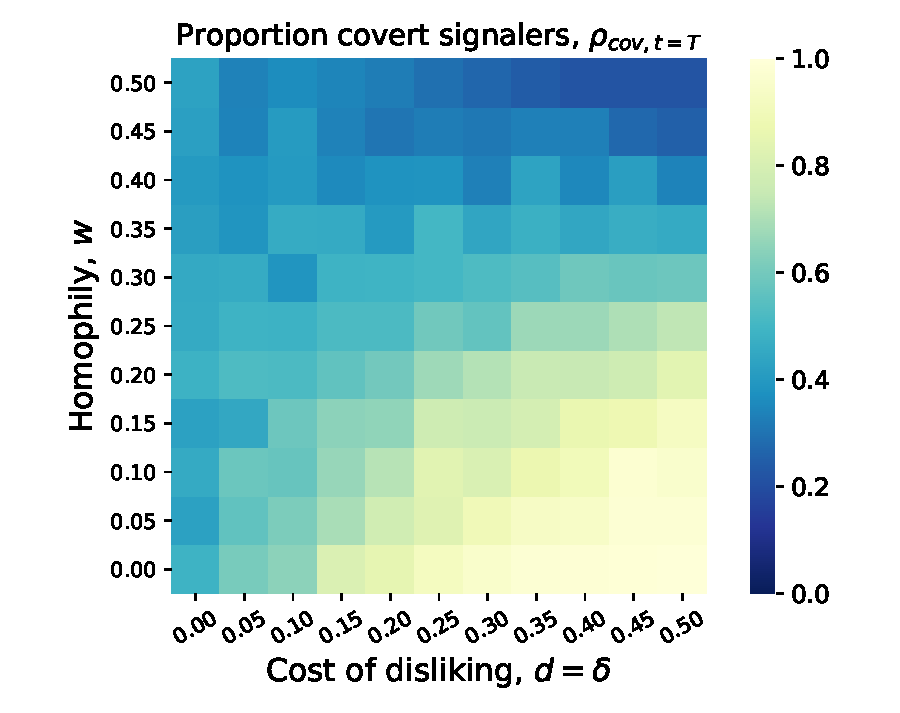
\includegraphics[width=\textwidth]{Figures/basic_disliking_signaling.pdf}
    \caption{Covert signaling prevalence under a variety of homophily and
    disliking penalty parameter values. }
  \end{subfigure}
  \begin{subfigure}{0.49\textwidth}
    \centering
    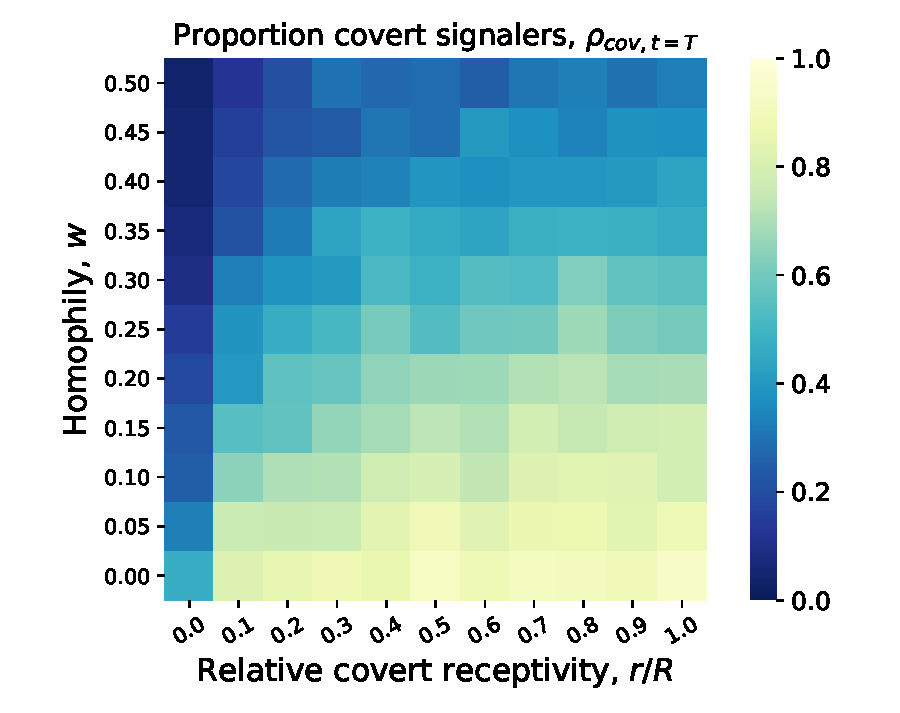
\includegraphics[width=\textwidth]{Figures/basic_receptivity_signaling.pdf}
    \caption{Covert signaling prevalence under a variety of homophily and
    covert signaling efficiency values. $d=0.25$; all other parameters set to
  defaults listed in Table~}
  \end{subfigure}
  
  \caption{Covert signaling prevalence is sensitive to changes in all 
  three explanatory parameters for our basic experiment, homophily ($w$),
disliking penalty ($d$), and covert signaling efficiency ($E_{cov}$). 
In (a) $E_{cov}=0.25$; in (b) $d=0.25$. All other parameters in both sets of 
    results (a) and (b) are set to defaults listed in Table~\ref{tab:params}.}
  \label{fig:dislikingHomophilyHeatmap}
\end{figure}

% \subsubsection{...as a function of covert signaling efficiency}


\subsubsection{Co-evolution of covert signaling and generous receiving}

(DID NOT YET GET TO RE-DO CORRELATIONS AND WRITE THIS SECTION)

% Theoretically, conditions favorable for covert
% signalers should also be favorable for generous receivers (TRUE??). Furthermore, 
% an increase in covert signalers increases the pressure towards generous receiving.
% With many covert signalers it is likely an agent will get no signal on a 
% turn because they were receiving a signal from a covert signaler. Disliking
% incurs a penalty, so it is better to remain neutral.


\begin{figure}[H]
  \centering
  \begin{subfigure}{0.49\textwidth}
    \centering
    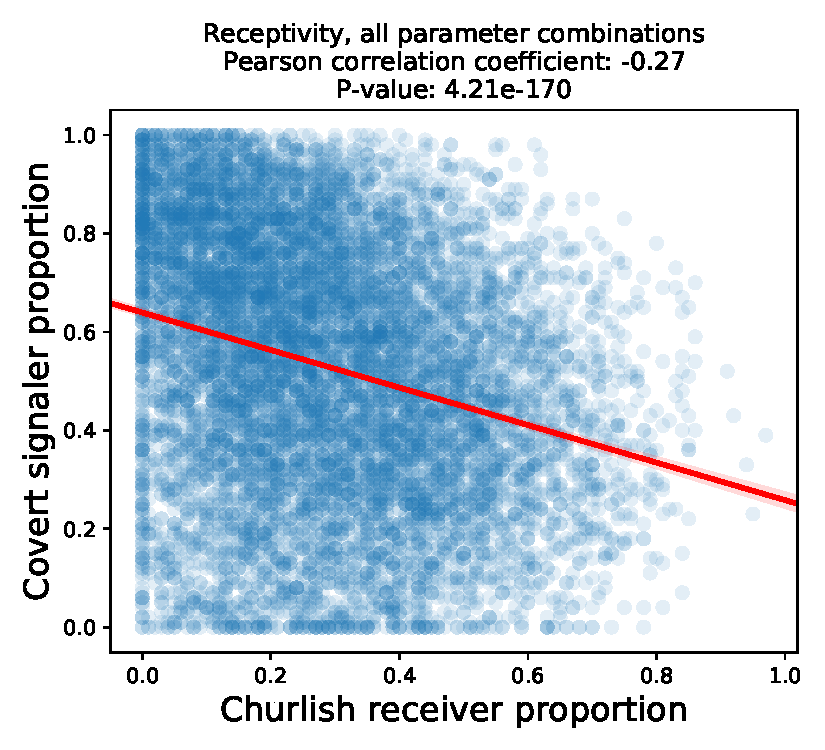
\includegraphics[width=\textwidth]{Figures/receptivity_allcombos_reg.pdf}
    \caption{}
    \label{fig:}
  \end{subfigure}
  \begin{subfigure}{0.49\textwidth}
    \centering
    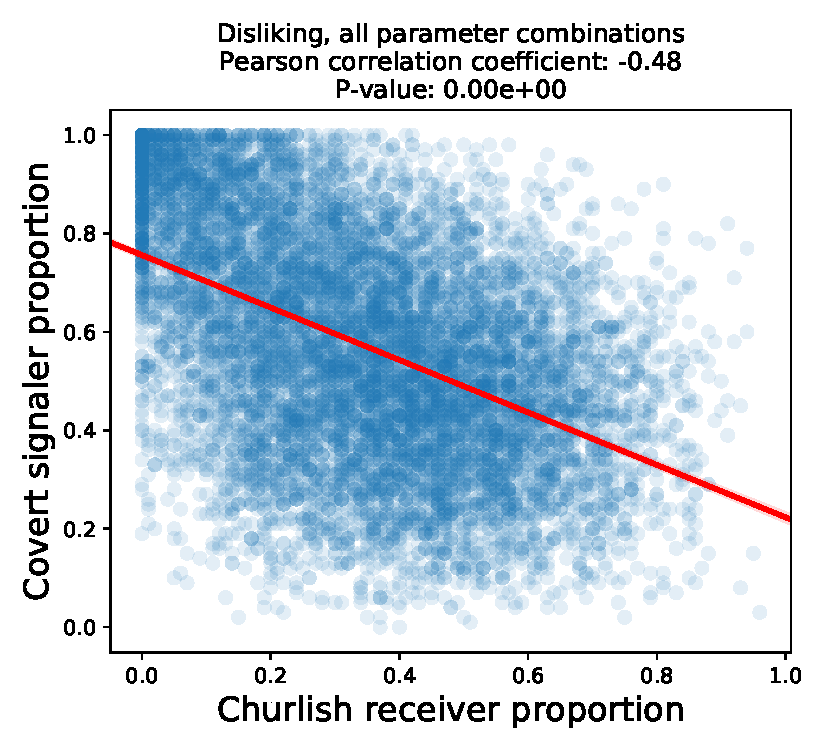
\includegraphics[width=\textwidth]{Figures/disliking_allcombos_reg.pdf}
    \caption{}
    \label{fig:}
  \end{subfigure}
  \caption{Correlation between proportion of covert signalers and proportion of
    churlish receivers for all tested parameter combinations in both 
    receptivity (a) and disliking (b) experiments. (NEED TO CHECK HOW I'M AVERAGING
    HERE AND POSSIBLY AGGREGATE FURTHER AS A SMOOTHING FILTER. ALSO NEED TO
). (THINK ABOUT HOW WE COULD USE PAIR PLOT GRIDS TO COMMUNICATE SOME OF
These, such as in https://jakevdp.github.io/PythonDataScienceHandbook/04.14-visualization-with-seaborn.html
I'm already going towards that with the invasion plots, but this would be
plotting correlations between outcome variables and maybe do a 2x2 with
signaling and receiving prevalences on x and y axes, respectively. Each plot
with be one of $s \in {cov, ov} \times {ch, gen}$.)}
  
  \label{fig:regressions}
\end{figure}

\subsubsection{Complex relationship between similarity threshold, homophily, and covert signaling}

(BELOW IS PRELIMINARY/OUTLINE TEXT TO UPDATE)

Now we evaluate two related hypotheses, that (1) more tolerant societies
foster greater overt signaling prevalence and less covert signaling, i.e., more
tolerant societies promote honest communication; 
and (2) increased cultural diversity fosters increased 
covert signaling prevalence---that is, one must be more cautious since more
diversity means more social norms and taboos to navigate. 

To test the first hypothesis that less tolerant societies foster greater
covert signaling prevalence, we
systematically varied the similarity threshold $S \in \{0.1, 0.2, \ldots, 0.9\}$.
Recall this threshold determines whether
two agents are deemed ``similar''. Two agents are similar if their similarity
$s_{ij} \geq S$ (see Equation~\ref{eq:similarity}; Table~\ref{tab:params}). 
We can think of the ``tolerance'' of agents to be $1-S$; then
high levels of tolerance mean a lower threshold for similarity. 

We found that covert signaling is indeed sensitive to the similarity threshold, 
$S$. In most cases, increased $S$ leads to increased covert signaling
prevalence. However, when homophily is high, increased $S$ leads to increased
\emph{overt}, not covert, signaling prevalence. This is understandable by
considering the interaction process composed of two phases, matching and
collaboration. Matching is totally random---all 100 agents are paired into
50 random dyads. Collaboration occurs probabilistically with the chance of
collaboration increasing with the attitudes each agent has towards the other.

To understand why overt signaling is sometimes favored over covert signaling,
consider the default situation, which we used in our
computational experiments. Covert signaling is
half as efficient than overt signaling, which is set to $E_{ov} = 2E_{cov} = 0.5$. 
Recall this means that when an agent signals, half of all other agents receive
an overt signal and one quarter receive a covert signal. Say a dyad is formed
where the agents are similar, but covert signalers and generous receivers
so they each have an attitude of 0 about the other, $a_{ij} = a_{ji} = 0$. 
There is a high probability that both agents do not get a signal about the other
in a given round of communication: $\frac{1}{4} \cdot \frac{1}{4} = \frac{1}{16}$.
The probability of collaboration is $\frac{1}{2}$ in this situation 
(Equation~\ref{eq:homophily}). If instead both agents were 
overt signalers the chance they like one another is $\frac{1}{4}$ and if
$w=0.5$ they are guaranteed to collaborate and reap a payoff of $1 + s$. 
If just one likes the other, the chance they collaborate is $\frac{3}{4}$
instead of $\frac{1}{2}$. There is a much higher chance of payoff if agents
know they like one another. We will see that this same pattern is inverted for
minority group agents when homophily is high so that they have a fighting chance to
get a payoff with a majority group agent they would likely be matched with. 

What to show with figures
\begin{itemize}
  \item In most all cases, when the similarity threshold reaches a large enough 
    value, covert signaling dominates. Exception is $K=3$ and $K=5$ with 
    $w=0.5$. When homophily is not maximal ($w \leq 0.4$) an increased 
    similarity threshold tends to increase covert signaling prevalence. 
    We consider $w=0.5$ and other select exceptions to this pattern later; 
    for now, we focus on showing this general trend of increased covert signaling
    with increased similarity (Figure~\ref{fig:covertAndSimilarity}).
  \item Unexpectedly, for moderately high levels of $S$ and high $w$, overt signaling is
    favored. As showed in previous result this goes away when $S$ gets to
    maximal values. However, for maximal $S=1.0$ and $w=0.5$ covert signaling
    does not come to dominate. When $K=3$, overt signaling becomes more
    preferred when $S$ goes from $0.5$\footnote{For $K=3$, $S=0.5$ is equivalent
        to $S=0.4$ and $S=0.6$---all refer to the situation where a pair matches
    two of three traits. For $K=5$, $S=0.5$ is only equivalent to $S=0.6$.}
    to $0.8$. For $K=5$, covert signaling prevalence recovers somewhat going
    from $S=0.7,0.8$ to $S=0.9,1.0$ (Figure~\ref{fig:overtAndSimilarity}).
  \item Worthwhile to note that when the disliking penalty is high and $S$ is low, 
      overt signaling is weakly favored for $w=0.3$. There also seems to be a
      weak effect at $w=0.4$ that is like dominance of overt signaling for
      moderate-high $S$ with maximal $w=0.5$.
      (GIVE DETAILS IN SUPPLEMENT \ref{fig:similarity_supp}) 
\end{itemize}

\begin{figure}
  \centering
  \large{Low to moderate homophily, $w=0.2$}
  \includegraphics[width=0.8\textwidth]{Figures/similarity/similarity_low_medium_S_homophily.pdf}
  \caption{When homophily is low to moderate ($0.0 \leq w \leq 0.3$), covert signaling
  prevalence increases monotonically with similarity threshold, $S$.}
  \label{fig:covertAndSimilarity}
\end{figure}

\begin{figure}
  \centering
  \large{High homophily, $w=0.5$}
  \includegraphics[width=0.8\textwidth]{Figures/similarity/similarity_high_S_homophily.pdf}
  \caption{
      When homophily is maximal ($w=0.5$) and $K$ is small (top row,
      $K=3$ and $K=5$), covert signaling
      prevalence is \emph{negatively} correlated with increased similarity 
      threshold, meaning larger $S$ favors \emph{overt}, not covert signaling. 
      This also occurs for maximal homophily and larger values of $K$, but 
      only to a point (bottom row). For larger values of $K$, $\rho_{cov}$
      decreases at first with $S$, but then undergoes a sudden transition to
      $\rho_{cov} \approx 1.0$.
  }
  \label{fig:overtAndSimilarity}
\end{figure}




\subsubsection{Evolution of signaling strategy in minority and majority groups}

Here we analyze the evolution of covert signaling in populations where there
are minority and majority sub-populations, as specified by agents' trait
vectors, $\tau_i$. In these experiments, the first $M$ of each agent's $K$ traits
are set to 1 or -1: fraction $\rho^{minor}$ of the
population is in the minority, and have the first $M$ of their traits set to
1, and the rest of the population is the majority, with the first $M$ of their
traits set to -1. 

We primarily vary the minority prevalence, $\rho^{minor} \in \{0.1, 0.15, \ldots, 0.45\}$. 
We vary $\rho^{minor}$ for two parameter pairs of $(K, M)$, where $K$ is the cultural 
complexity, and $M$ is the integer number of traits used to define 
majority/minority populations. The similarity threshold is set to $S=0.5$. 
We test the settings $K=3$, $M=1$, and $K=9$, $M=4$. We also test three
values of homophily and disliking penalty, representing low, medium, and high
levels for each: $w,d \in \{0.05, 0.25, 0.45\}$.

We found (SUPPORTED BY FIGURES)\dots
\begin{itemize}
    \item Basic results (FIRST FIGURE)
        \begin{itemize}
          \item High levels of homophily and low costs for disliking favor 
              decreased covert signaling prevalence among minority for 
              $S=0.5$ (Figures: all conditions
              with $S=0.5$)
          \item Larger minority population size decreases covert 
              signaling prevalence among the minority,
            but weakly if at all---would want to integrate over $d$, $w$ values.
            (Compare, e.g., K=9, S=0.5, and $\rho^{minor}=0.1,0.2$).
          \item Increased overall diversity (increased $K$) increases prevalence of 
            covert signaling among minority for low to moderate 
            similarity thresholds (Figures: compare $K=3,9$ over 
            $S=0.3, 0.5$---Four plots---TWO ALREADY THERE,
            PUT S=0.3 IN SUPPLEMENT).
        \end{itemize}
  \item High levels of homophily and similarity threshold favor covert signaling.
    (Figures: selection of two figures where $S=0.8$ SECOND FIGURE IN MAIN TEXT)
\end{itemize}

(ALL FIGURES BELOW WERE RUN PRELIMINARY WITH 20 TRIALS. I HAVE DATA FOR 100
TRIALS BUT HAVE NOT YET ANALYZED IT)

\begin{figure}
  \centering
  \begin{subfigure}{0.49\textwidth}
      \includegraphics[width=\textwidth]{Figures/minority_tolerance/3_0p10_0p5.pdf}
      \caption{}
    \end{subfigure}
    \begin{subfigure}{0.49\textwidth}
      \includegraphics[width=\textwidth]{Figures/minority_tolerance/9_0p10_0p5.pdf}
      \caption{}
    \end{subfigure} \\[1em]
    \begin{subfigure}{0.49\textwidth}
      \includegraphics[width=\textwidth]{Figures/minority_tolerance/3_0p20_0p5.pdf}
      \caption{}
      \end{subfigure}
    \begin{subfigure}{0.49\textwidth}
      \includegraphics[width=\textwidth]{Figures/minority_tolerance/9_0p20_0p5.pdf}
      \caption{}
    \end{subfigure}
    \caption{When homophily is high, disliking costs are low, and
      similarity threshold is moderate ($S=0.5$ in these heatmaps), covert 
    signaling is more common among the majority than the minority. When 
  disliking costs are high and homophily is not, covert signaling is more
prevalent among the minority than the majority. Results shown from condition
where $\rho^{minor}=0.1$. We observe the same pattern with $\rho^{minor}=0.2$
(Figure~\ref{fig:suppBasicMinorityResult}). All parameters not specified are set
to their default values (Table~\ref{tab:params}).}
  \label{fig:}
\end{figure}


\begin{figure}
  \centering
  \begin{subfigure}{0.49\textwidth}
      \includegraphics[width=\textwidth]{Figures/minority_tolerance/3_0p10_0p8.pdf}
      \caption{}
    \end{subfigure}
    \begin{subfigure}{0.49\textwidth}
      \includegraphics[width=\textwidth]{Figures/minority_tolerance/9_0p10_0p8.pdf}
      \caption{}
    \end{subfigure}
    \caption{A high similarity threshold ($S=0.8$ here) promotes covert
    signaling differentially among the minority when homophily is also high.
    Here $\rho^{minor}=0.1$, but the same pattern is also observed for 
  $\rho^{minor}=0.2$ (NEED TO PUT IN A SUPPLEMENT FIGURE~\ref{fig:highSimilarityHomophily_supp}).}
  \label{fig:highSimilarityHomophily}
\end{figure}


% \begin{figure}
%   \centering
%   \begin{subfigure}{0.49\textwidth}
%       \includegraphics[width=\textwidth]{Figures/minority_tolerance/3_0p10_0p5.pdf}
%       \caption{}
%     \end{subfigure}
%     \begin{subfigure}{0.49\textwidth}
%       \includegraphics[width=\textwidth]{Figures/minority_tolerance/9_0p10_0p5.pdf}
%       \caption{}
%     \end{subfigure}
%     \caption{When homophily is high, disliking costs are low, and
%       similarity threshold is moderate ($S=0.5$ in these heatmaps), covert 
%     signaling is more common among the majority than the minority. When 
%   disliking costs are high and homophily is not, covert signaling is more
% prevalent among the minority than the majority. Results shown from condition
% where $\rho^{minor}=0.1$. We observe the same pattern with $\rho^{minor}=0.2$
% (Figure~\ref{fig:suppBasicMinorityResult}). All parameters not specified are set
% to their default values (Table~\ref{tab:params}).}
%   \label{fig:}
% \end{figure}

% % \subsubsection{Covert minority signaling over minority prevalence}


% % \begin{figure}[H]
% %   \centering
% %   \begin{subfigure}{0.48\textwidth}
% %     \centering
% %     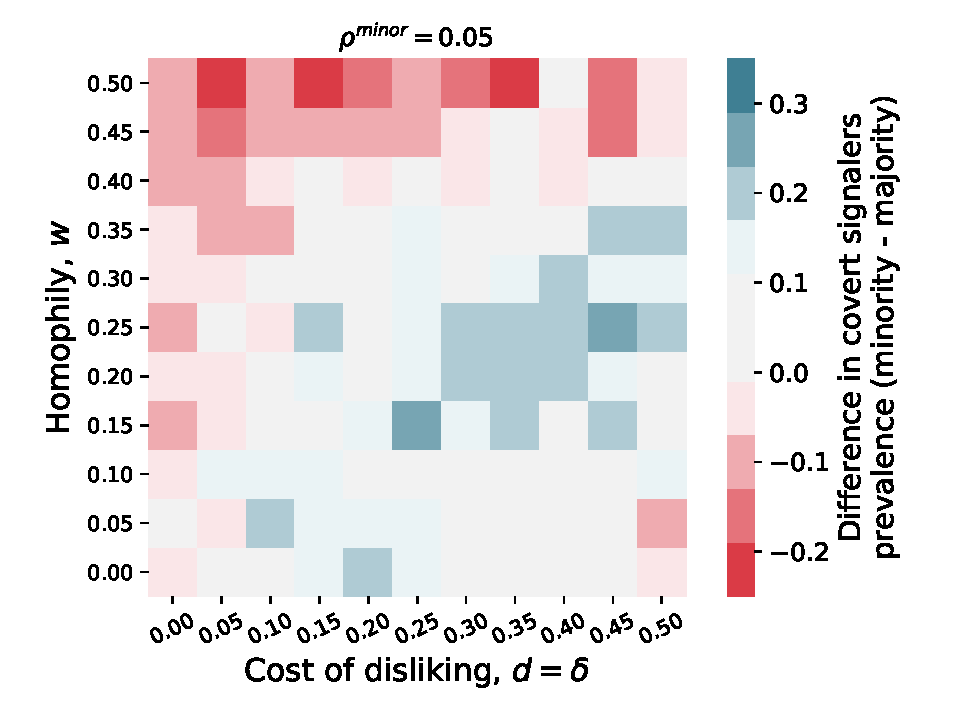
\includegraphics[width=\textwidth]{Figures/covert_signalers_diff_0p05.pdf}
% %     % \caption{Prevalence of minority covert receivers; $\rho^{minor} = 0.10$.}
% %   \end{subfigure}
% %   \hfill
% %   \begin{subfigure}{0.48\textwidth}
% %     \centering
% %     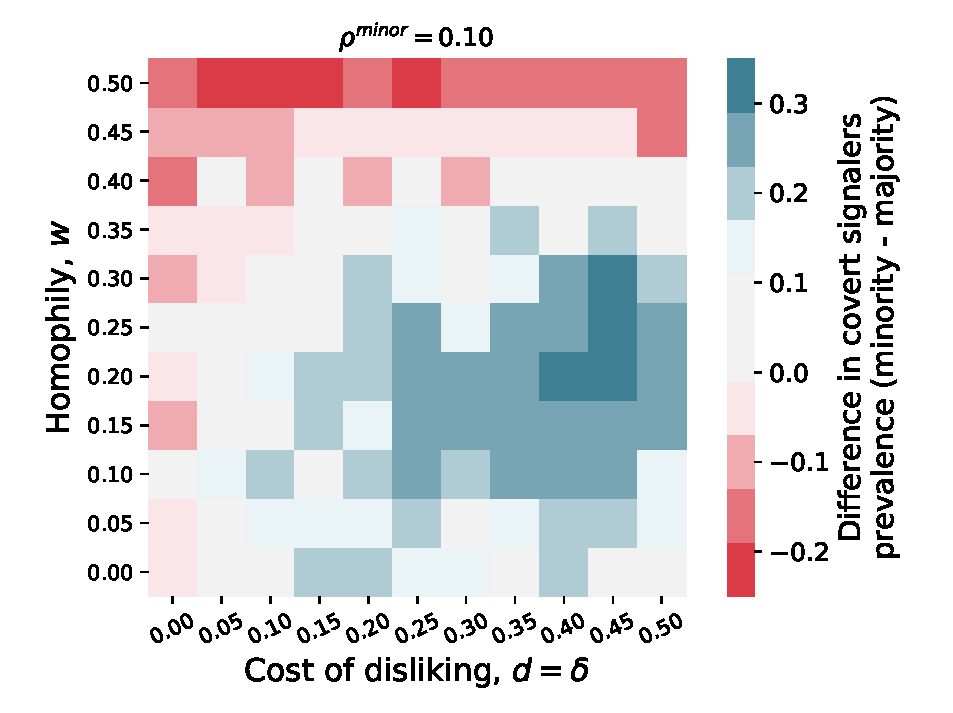
\includegraphics[width=\textwidth]{Figures/covert_signalers_diff_0p10.pdf}
% %     % \caption{Prevalence of minority covert receivers; $\rho^{minor} = 0.25$.}
% %   \end{subfigure} \\[.25in]
% %   \begin{subfigure}{0.48\textwidth}
% %     \centering
% %     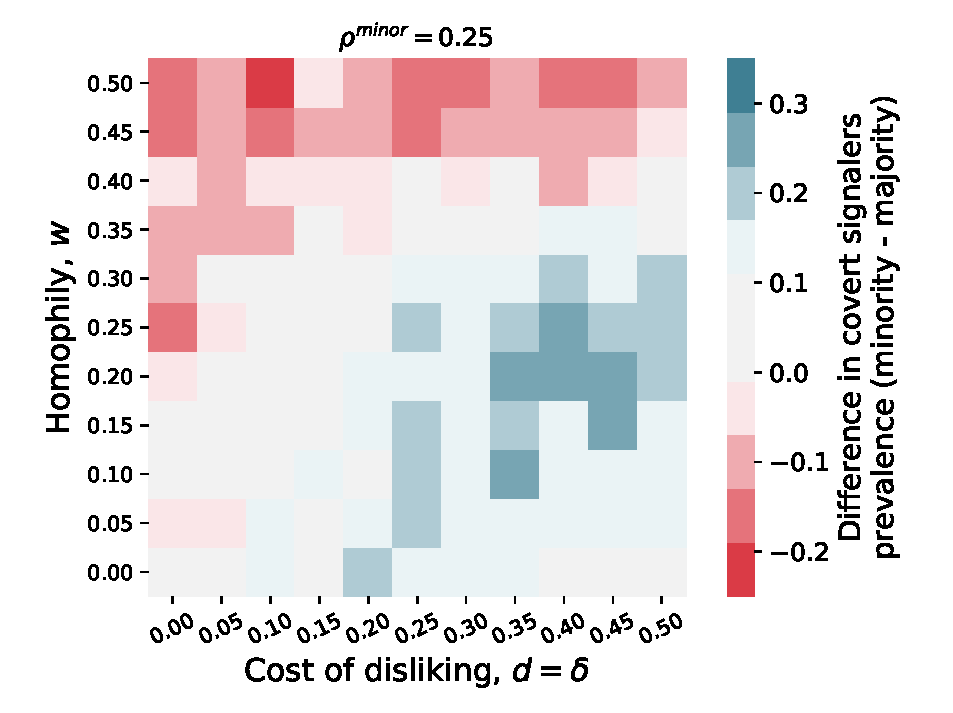
\includegraphics[width=\textwidth]{Figures/covert_signalers_diff_0p25.pdf}
% %     % \caption{Prevalence of minority churilsh receivers; $\rho^{minor} = 0.10$.}
% %   \end{subfigure}
% %   \hfill
% %   \begin{subfigure}{0.48\textwidth}
% %     \centering
% %     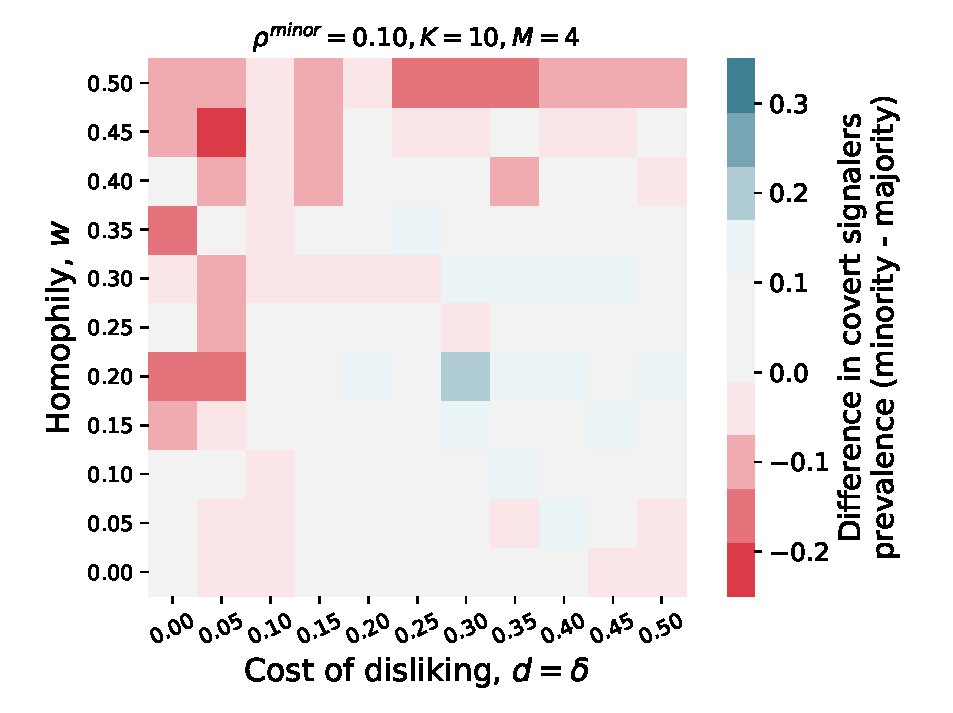
\includegraphics[width=\textwidth]{Figures/covert_signalers_diff_0p10_K=10_M=4.pdf}
% %     \caption{(NEED TO UPDATE WITH K=9 AND M=4. Ran these, just need to pull from
% %     MERCED and analyze.)}
% %   \end{subfigure}
% %   \caption{Difference in covert signaling prevalence between minority and
% %   majority populations for different parameters settings.}
% %   \label{fig:covert-signaling-minority-heatmap}
% % \end{figure}

% \begin{figure}[H]
%   \centering
%   \begin{subfigure}{0.31\textwidth}
%     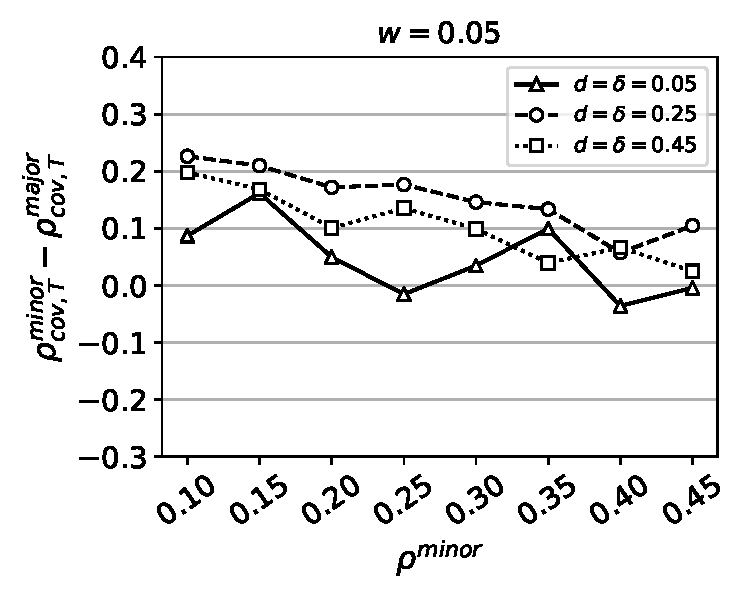
\includegraphics[width=\textwidth]{Figures/minority-homophily=0p05.pdf}
%     \caption{}
%   \end{subfigure}
%   \begin{subfigure}{0.31\textwidth}
%     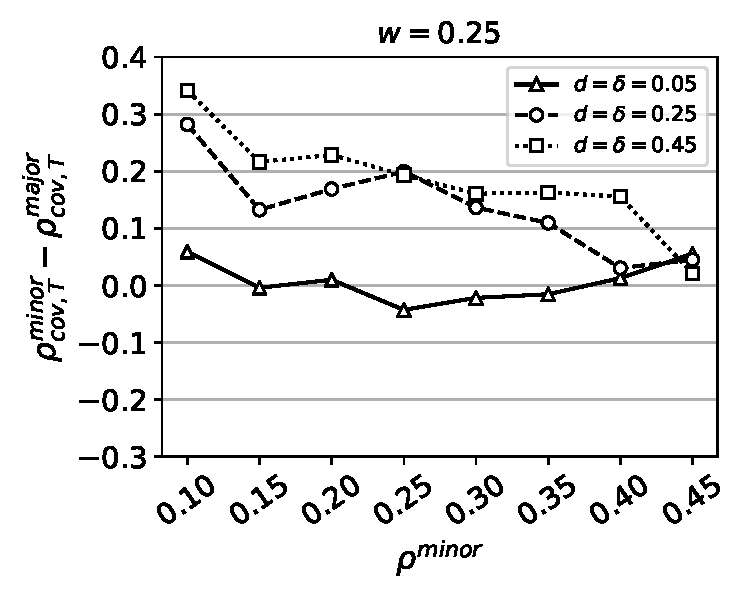
\includegraphics[width=\textwidth]{Figures/minority-homophily=0p25.pdf}
%     \caption{}
%   \end{subfigure}
%   \begin{subfigure}{0.31\textwidth}
%     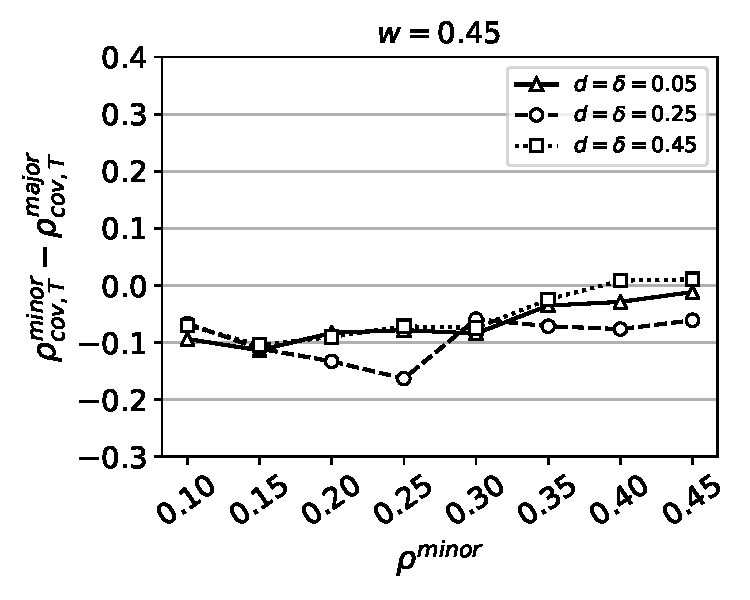
\includegraphics[width=\textwidth]{Figures/minority-homophily=0p45.pdf}
%     \caption{}
%   \end{subfigure}
%   \caption{}
% \end{figure}



\subsection{Covert signaling invasion}

In this experiment we begin with initial proportions, $\rho$ of one of the strategies
at 0.05 and consider this the ``invading'' strategy. $\rho_{cov,0}$ represents
the initial covert proportion, $\rho_{ov,0}$ the initial overt proportion,
$\rho_{ch,0}$ the initial churlish proportion, and $\rho_{gen,0}$ the 
initial generous proportion. We measure how often
a non-zero proportion of agents with the invading strategy manage to 
establish a permanent population, which we call invasion success. We calculated
invasion success for a number of experimental parameter settings, covarying
over disliking penalty ($d=\delta$) and homophily ($w$) in the first case,
and over relative covert receptivity ($r/R$) and homophily ($w$) 
in the second case (Figure~\ref{fig:cov-invades} below; Figures~\ref{fig:ov-invades} and~\ref{fig:ch-gen-invades} in the supplement).

\begin{figure}[H]
  \centering
  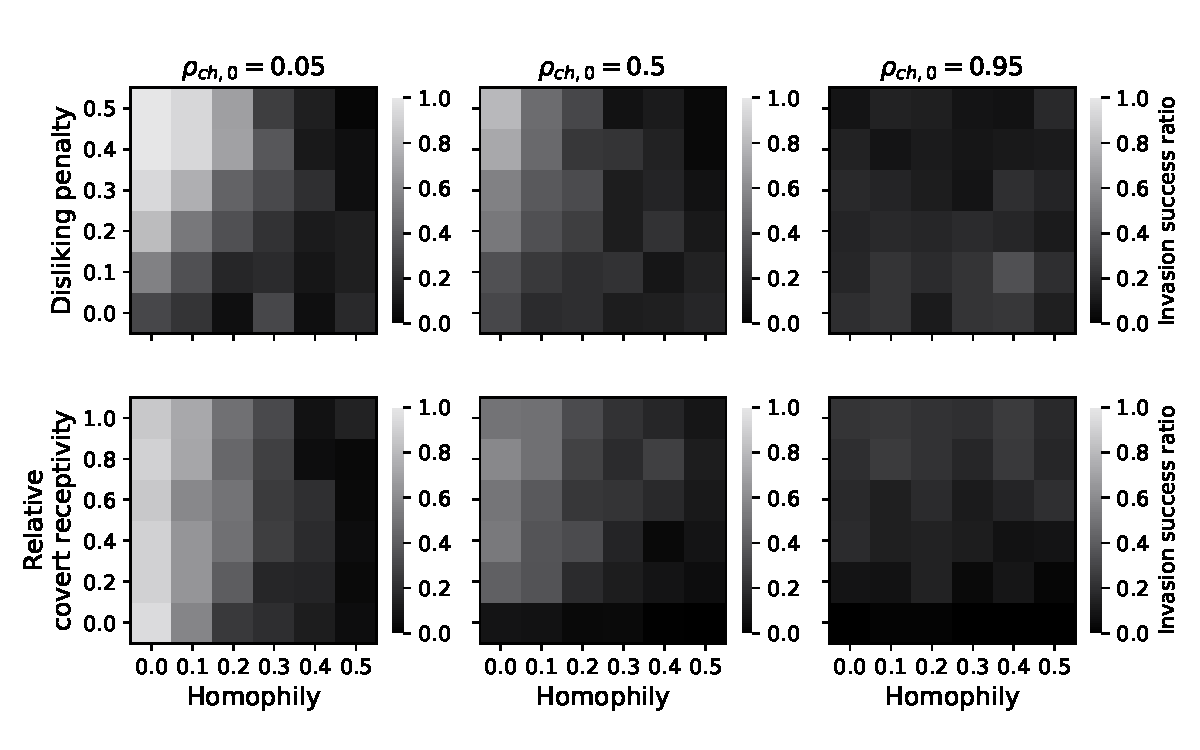
\includegraphics[width=\textwidth]{Figures/covert_invades.pdf}
  % \caption{Covert invades, $\rho_{cov,0}=0.05$}
  \caption{Covert and overt sending strategy invasion success rates. 
    Lower homophily is more favorable for successful covert signaling invasion.
    This is due to lower homophily meaning agents cannot assort well into
    similar pairs prior to interaction.
    Similarly, greater homophily is more favorable for successful overt
    signaling invasion, where agents can better assort if they know each other's
    true traits. Unexpectedly, as covert receptivity increases, overt signaling
    is is more successful at invading and covert signaling is less successful
    at invading when the initial churlishness is high. When initial
    churlishness is small to moderate, the pattern is reversed.
  }
  \label{fig:cov-invades}
\end{figure}


\subsubsection{Non-signaling as an adaptive strategy}

One of the most striking patterns in the invasion results is the evolution
of a third de facto strategy of non-signaling. This strategy emerges when
we consider both the invasion dynamics of either the covert or overt 
signaling strategy. When simulating the invasion of covert signaling
($\rho_{cov,0}=0.05$), the non-signaling strategy emerges when the covert
signaling efficiency, $r$, is 0, but covert signaling still successfully
invades as the chosen agent strategy. When $r=0$, no agents receive
covert signals, making this more accurately a \emph{non-signaling} strategy.  
For covert signaling invasion, this only happens when the initial churlishness
is low ($\rho_{ch,0}=0.05$) and homophily is also low ($w \lessapprox 0.2$). 
Non-signaling wins out evolutionarily 
in some cases when considering of invading overt signalers when overt signalers
fail to invade but $r=0$, again meaning agents in this society prefer not
to signal at all. This occurs some of the time for all tested homophily
values and low initial churlishness ($\rho_{ch,0}=0.05$) (Figure~\ref{fig:cov-invades}, bottom left plot).  
Overt signaling continues to fail to evolve at least some of the time
for $r=0$ for moderate initial churlishness ($\rho_{ch,0}=0.5$) up up to perfect 
assortment homophily, $w=0.5$.

\subsection{Further analyses and robustness checks}

There are a number of analyses that could be done to extend or check the 
robustness of the results presented here. In this section we present some
we deem most important and straightforward, and present more of these extensions
and checks in the supplement.

In this main text we present
\begin{itemize}
  \item Correlation between churlish receiving and covert signaling.
  \item Case where $\delta \neq d$---that is, the penalty from collaboration
    payoff is not $2d$ when both agents dislike one another, it is $d + \delta$.
  \item We check the robustness of our conclusions regarding covert signaling
    in minority populations by running our minority/majority
    experiments with $K=9$ instead of $K=3$ as we had above.
\end{itemize}

% \bibliographystyle{apacite}

% \setlength{\bibleftmargin}{.125in}
% \setlength{\bibindent}{-\bibleftmargin}

% \bibliography{/Users/mt/workspace/papers/library.bib}

\appendix

\section{Additional analyses}

\subsection{Similarity threshold experiment---further details}

\begin{figure}[H]
    \centering
  \label{fig:}
  \centering
  \begin{subfigure}{\textwidth}
    \centering
      \includegraphics[width=0.8\textwidth]{Figures/similarity_threshold_matrix_K=3.pdf}
      \caption{}
  \end{subfigure}
  \begin{subfigure}{\textwidth}
    \centering
      \includegraphics[width=0.8\textwidth]{Figures/similarity_threshold_matrix_K=5.pdf}
      \caption{}
  \end{subfigure}
  \caption{}
\end{figure}
\begin{figure}[H]
  \ContinuedFloat
    \centering
  \begin{subfigure}{\textwidth}
    \centering
      \includegraphics[width=0.8\textwidth]{Figures/similarity_threshold_matrix_K=9.pdf}
      \caption{}
  \end{subfigure}
  \begin{subfigure}{\textwidth}
    \centering
      \includegraphics[width=0.8\textwidth]{Figures/similarity_threshold_matrix_K=15.pdf}
      \caption{}
  \end{subfigure}
  \caption{}
\end{figure}
\begin{figure}[H]
    \ContinuedFloat
    \centering
  \begin{subfigure}{\textwidth}
    \centering
      \includegraphics[width=0.8\textwidth]{Figures/similarity_threshold_matrix_K=21.pdf}
      \caption{}
  \end{subfigure}
  \label{fig:similarity_supp}
  \caption{All results for experiments varying the similarity threshold, which
      could be thougth of as the additive inverse of tolerance. There are a
      number of subtle patterns described in detail in the main text and here
      in the supplement. Notably\dots (RECAP BRIEFLY HERE AND HIGHLIGHT 
      STUFF NOT INCLUDED IN MAIN).
}
\end{figure}


\subsection{Receiving strategy prevalence dynamics}

Recall that in our experiments, when agents learn they may adopt a new signaling 
strategy or receiving strategy.  In the main text we focused on covert 
signaling prevalence as a function of homophily, disliking penalty, and 
covert signaling efficiency. Here we support supplemental hypotheses about
the churlish recieving prevalence dynamics: (1) increased homophily tends
to increase the prevalence of churlish receivers; (2) churlish receiving
will be selected against when the disliking penalty is higher; and,
finally, (3) the prevalence of churlish receivers increases with 
covert signaling efficiency. 

(EXPLAIN IN MORE DETAIL)

\begin{figure}[H]
  \centering
  \begin{subfigure}{0.49\textwidth}
    \centering
    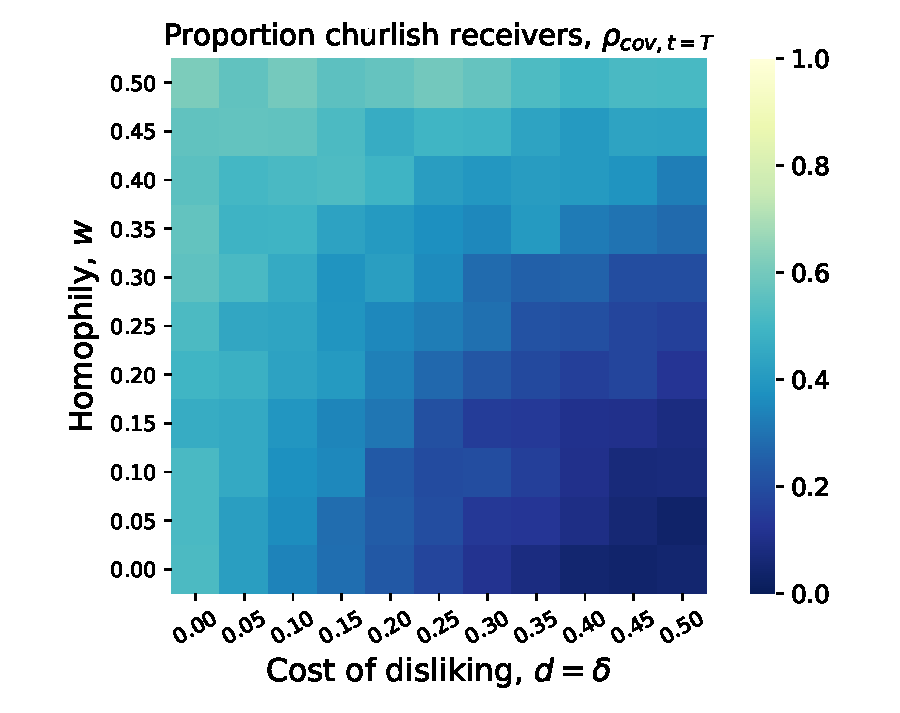
\includegraphics[width=\textwidth]{Figures/basic_disliking_receiving.pdf}
    \caption{Density of covert signalers.}
  \end{subfigure}
  \begin{subfigure}{0.49\textwidth}
    \centering
    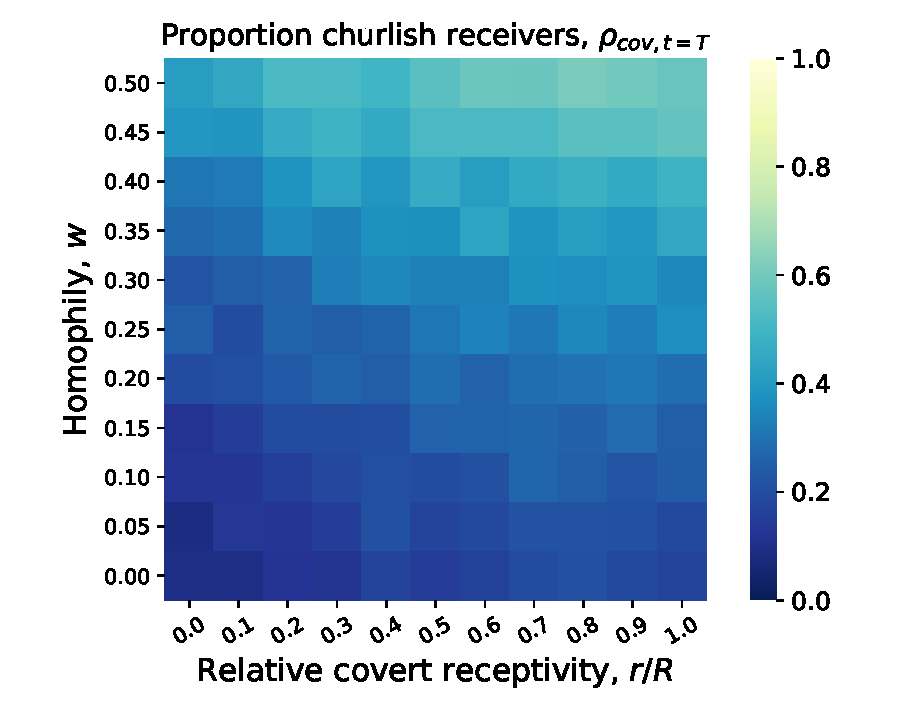
\includegraphics[width=\textwidth]{Figures/basic_receptivity_receiving.pdf}
    \caption{Density of churlish receivers.}
  \end{subfigure}
  
  \caption{Density of covert signalers and churlish receivers at $t=200$, 
    final timestep recorded in this preliminary experiment. Receptivity of
    overt signals is $R=0.5$. (THIS IS USING OLD DATA---NEED TO UPDATE WITH
    LATEST DATA USED TO GENERATE PLOTS ABOVE).}
  \label{fig:receptivityHomophilyHeatmap}
\end{figure}

\subsubsection{Minority churlish receiving over homophily and disliking}

In the main text we showed covert signaling is more prevalent in minority 
populations than the majority for most, but not all, parameter settings. 
Here we supplement this analysis by analyzing what conditions lead to
churlish receiving in the minority. (Reason out how it would benefit minority
agents to adopt churlish receiving).

(THESE ARE OLD RESULTS, NOT TAKEN FROM DATASETS USED TO MAKE CURRENT MAIN
TEXT SIGNALING STRATEGY RESULTS. NEED TO UPDATE THESE.)

\begin{figure}[H]
  \centering
  \begin{subfigure}{0.48\textwidth}
    \centering
    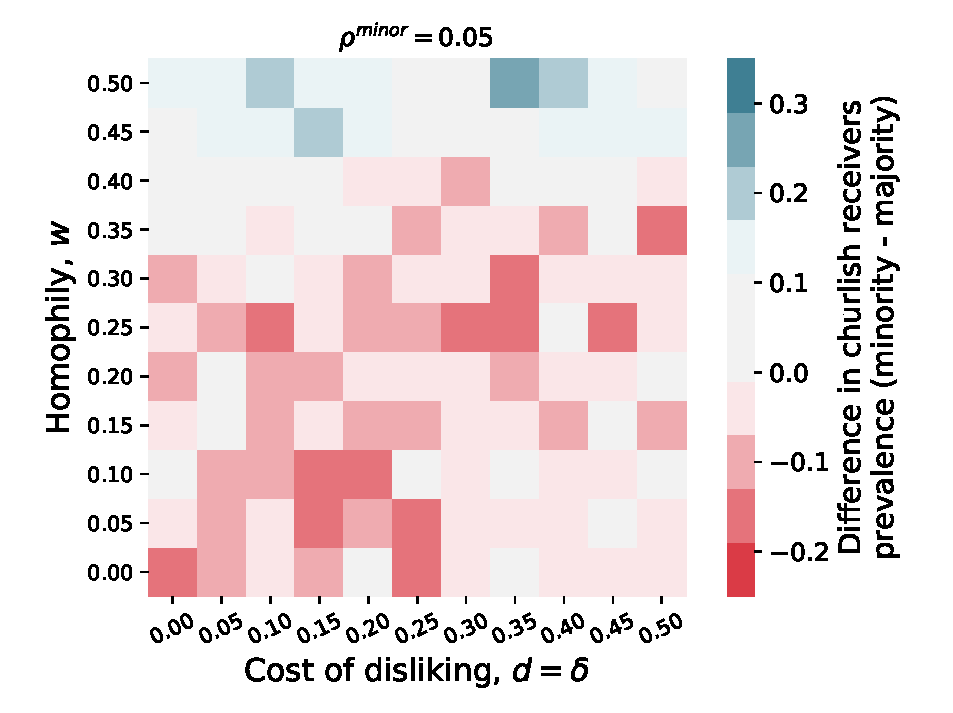
\includegraphics[width=\textwidth]{Figures/churlish_receivers_diff_0p05.pdf}
    % \caption{Prevalence of minority covert receivers; $\rho^{minor} = 0.10$.}
  \end{subfigure}
  \hfill
  \begin{subfigure}{0.48\textwidth}
    \centering
    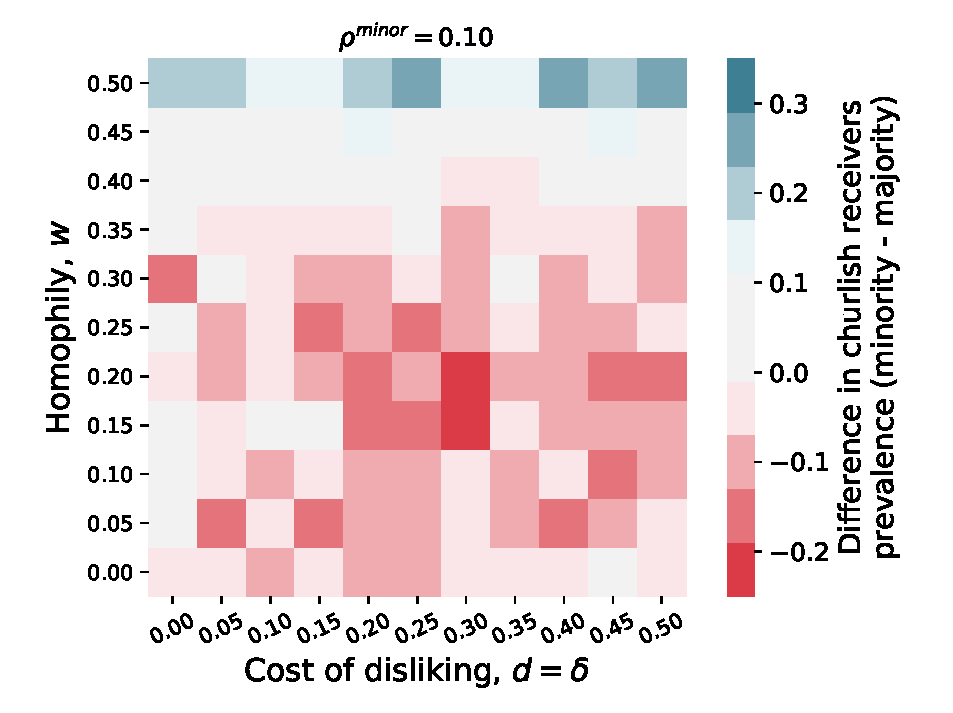
\includegraphics[width=\textwidth]{Figures/churlish_receivers_diff_0p10.pdf}
    % \caption{Prevalence of minority covert receivers; $\rho^{minor} = 0.25$.}
  \end{subfigure} \\[.25in]
  \begin{subfigure}{0.48\textwidth}
    \centering
    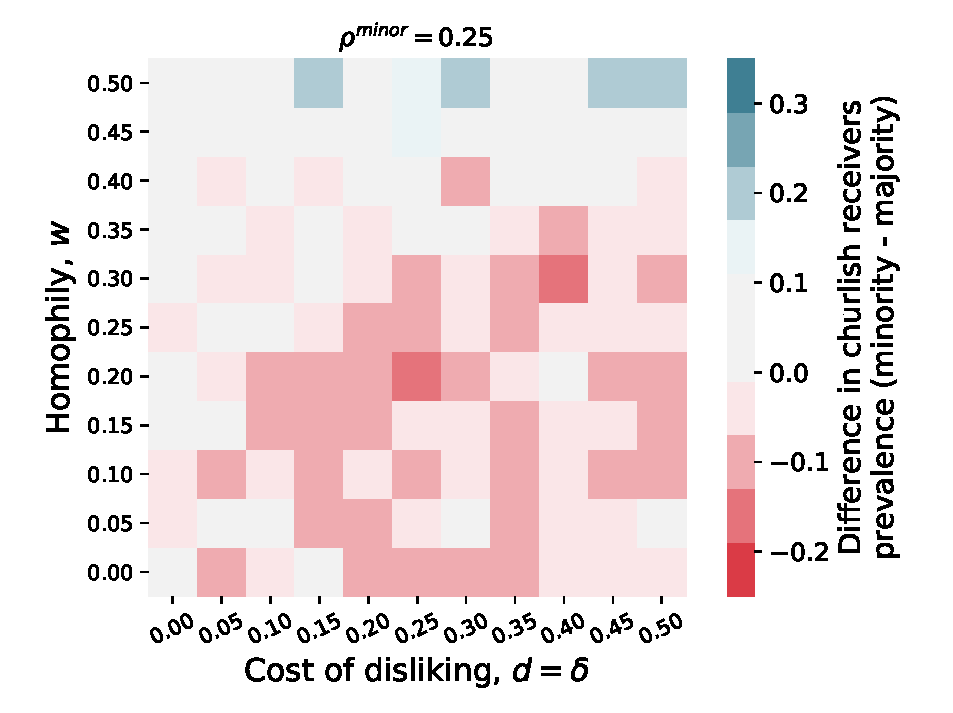
\includegraphics[width=\textwidth]{Figures/churlish_receivers_diff_0p25.pdf}
    % \caption{Prevalence of minority churilsh receivers; $\rho^{minor} = 0.10$.}
  \end{subfigure}
  \hfill
  \begin{subfigure}{0.48\textwidth}
    \centering
    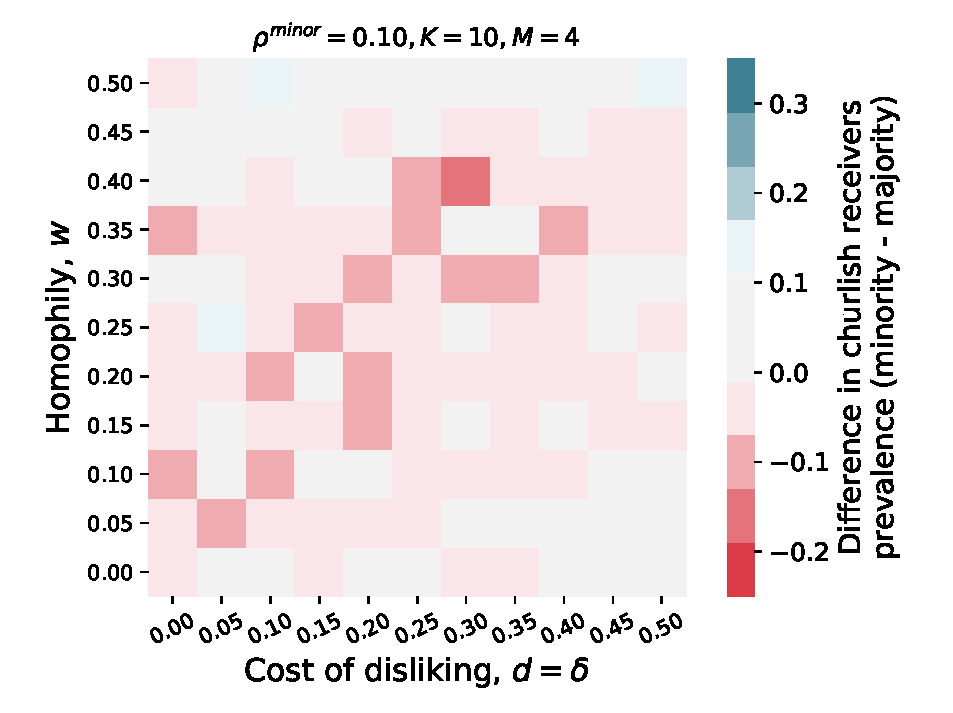
\includegraphics[width=\textwidth]{Figures/churlish_receivers_diff_0p10_K=10_M=4.pdf}
    % \caption{Prevalence of minority churilsh receivers; $\rho^{minor} = 0.25$.}
  \end{subfigure}
  \caption{Difference in churlish receiving prevalence between minority and majority
  populations for different parameter settings.}
\end{figure}

\subsection{Temporal dynamics and distribution of outcomes}

To understand how the model works it is important to examine ensembles and
means of time series for different parameter settings. In the results presented
in the main text, all reported values were calculated using the final
time step, where the time series had approximately reached equilibrium.
We want to be sure that the model actually reaches equilibrium.

We also want to know whether the mean of the outcomes is close to the
median value of the outcomes. That is, if the mean
final covert signaling prevalence is some value we want to be sure that
this is more an estimate of a typical prevalence value, not a measure of 
how often prevalence is either 0 or 1 at equilibrium.

\subsubsection{Temporal dynamics}

\begin{figure}[H]
  \centering
  \begin{subfigure}{0.49\textwidth}
    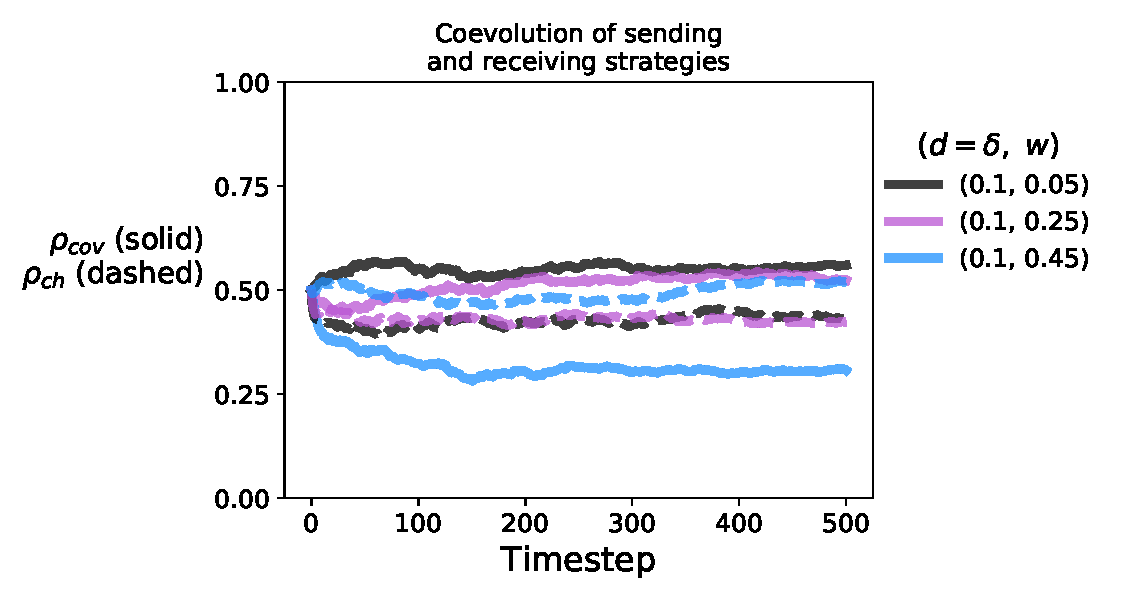
\includegraphics[width=\textwidth]{Figures/disliking_evo_d=0p1.pdf}
  \caption{}
  \end{subfigure}
  \begin{subfigure}{0.49\textwidth}
    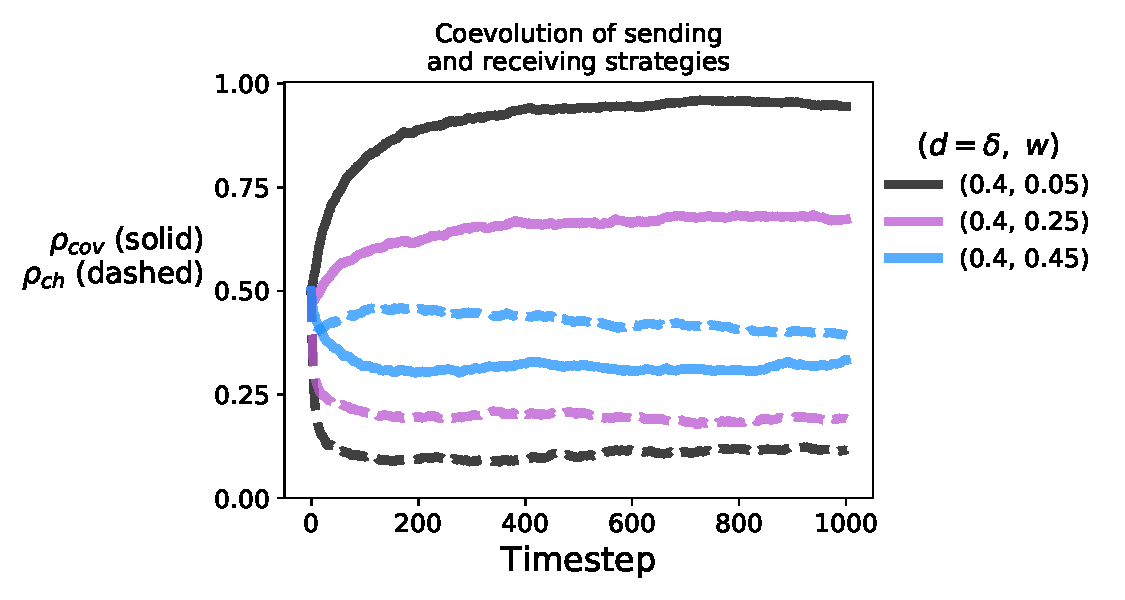
\includegraphics[width=\textwidth]{Figures/disliking_evo_d=0p4.pdf}
  \caption{}
  \end{subfigure} \\
  \begin{subfigure}{0.49\textwidth}
    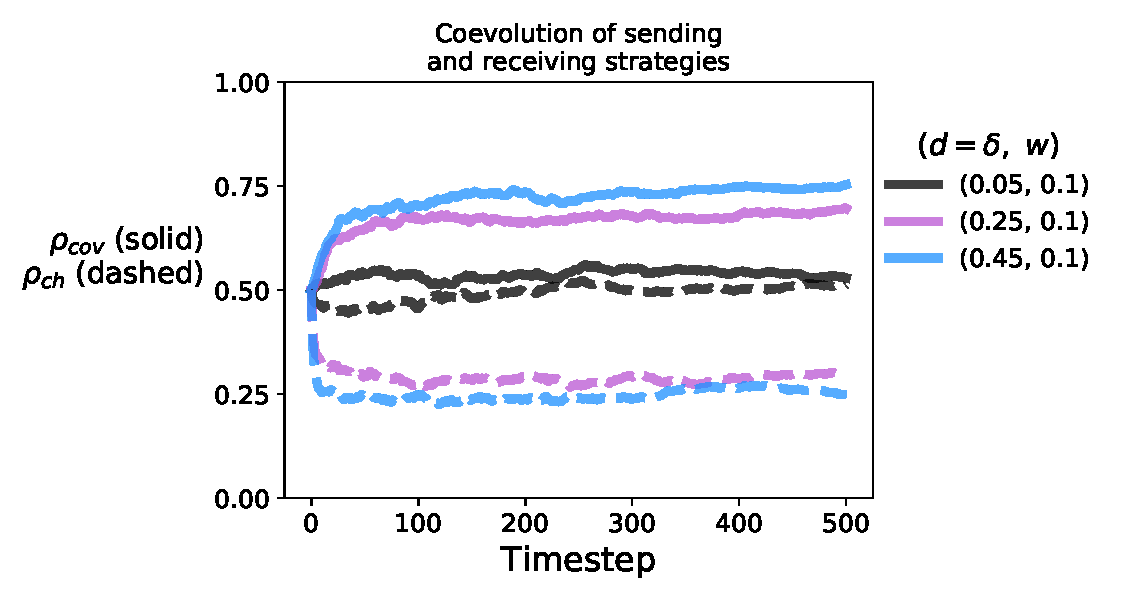
\includegraphics[width=\textwidth]{Figures/disliking_evo_w=0p1.pdf}
  \caption{}
  \end{subfigure}
  \begin{subfigure}{0.49\textwidth}
    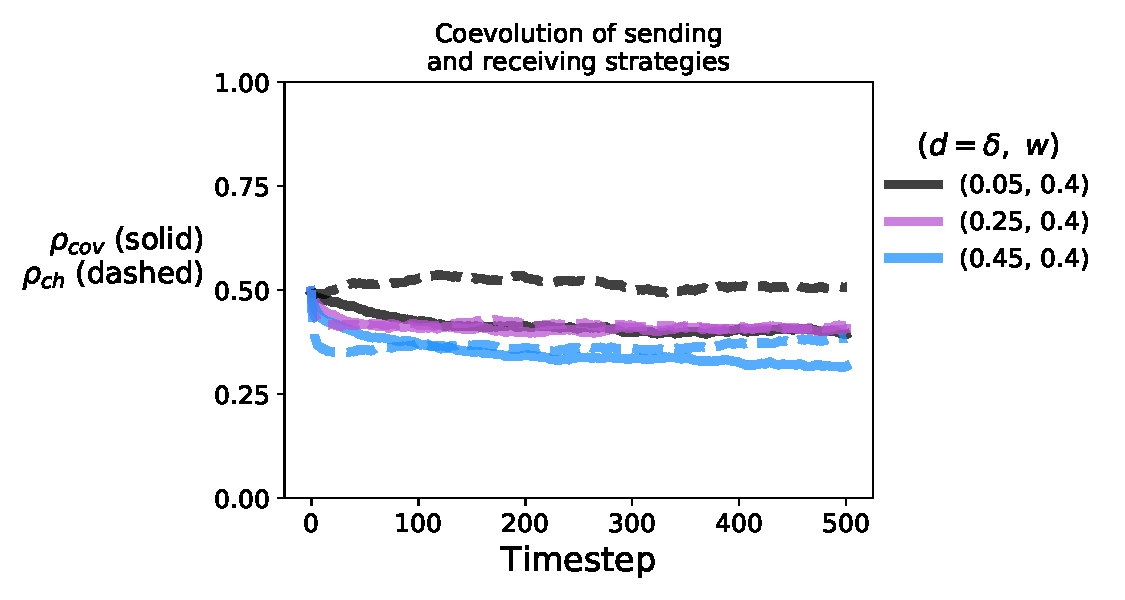
\includegraphics[width=\textwidth]{Figures/disliking_evo_w=0p4.pdf}
  \caption{}
  \end{subfigure}
  \caption{Time series of communication strategy prevalences under different parameter settings
  for homophily, $w$, and disliking penalty, $d$.}
  \label{fig:}
\end{figure}

\begin{figure}[H]
  \centering
  \begin{subfigure}{0.49\textwidth}
    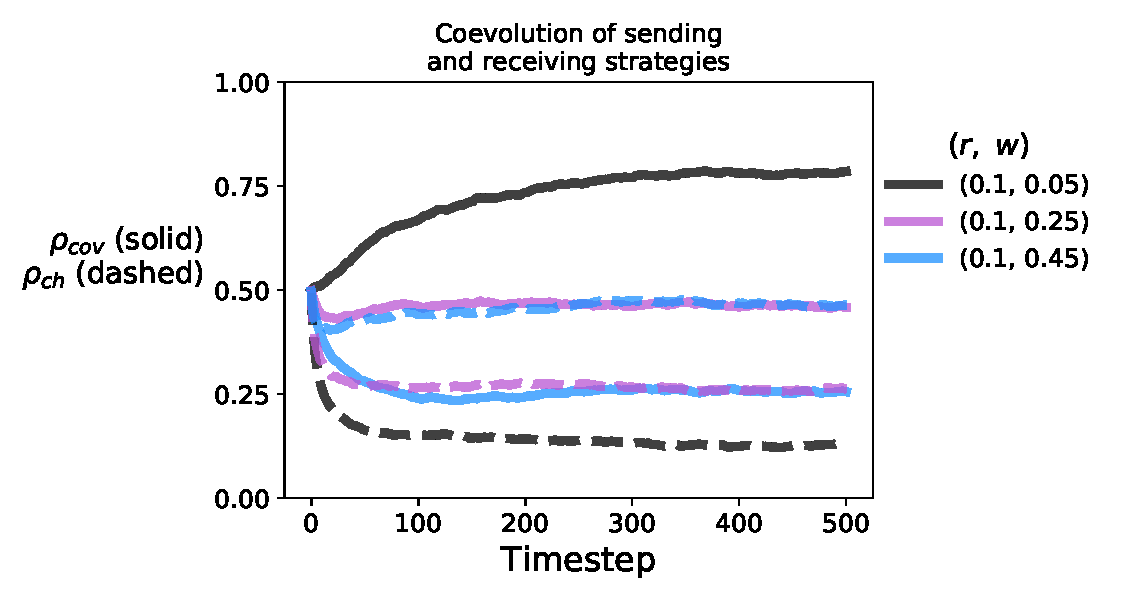
\includegraphics[width=\textwidth]{Figures/receptivity_evo_r=0p1.pdf}
  \caption{}
  \end{subfigure}
  \begin{subfigure}{0.49\textwidth}
    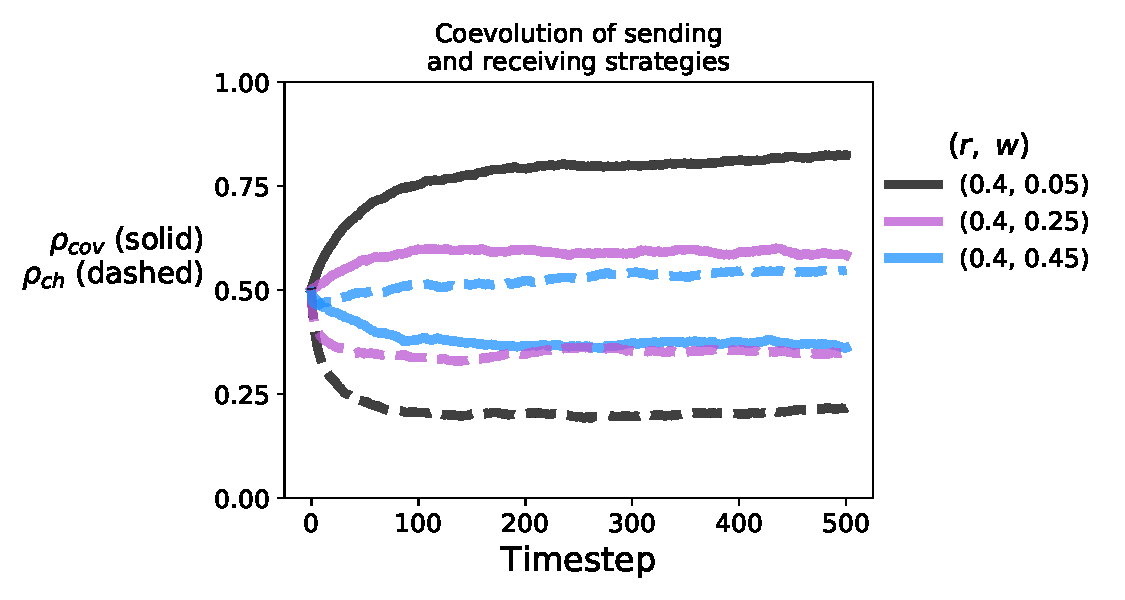
\includegraphics[width=\textwidth]{Figures/receptivity_evo_r=0p4.pdf}
  \caption{}
  \end{subfigure} \\
  \begin{subfigure}{0.49\textwidth}
    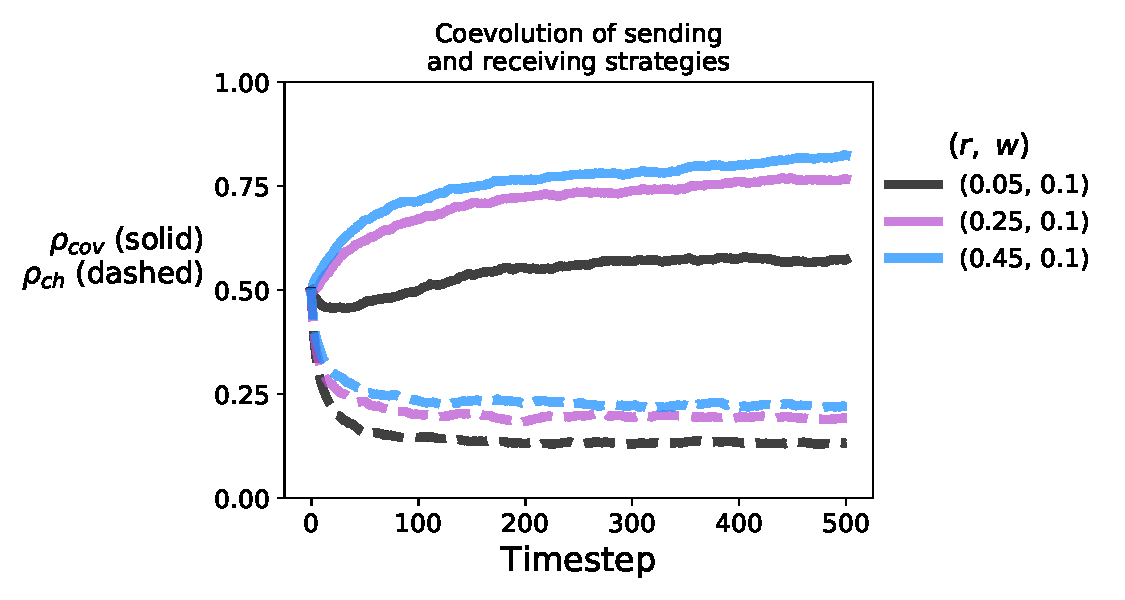
\includegraphics[width=\textwidth]{Figures/receptivity_evo_w=0p1.pdf}
  \caption{}
  \end{subfigure}
  \begin{subfigure}{0.49\textwidth}
    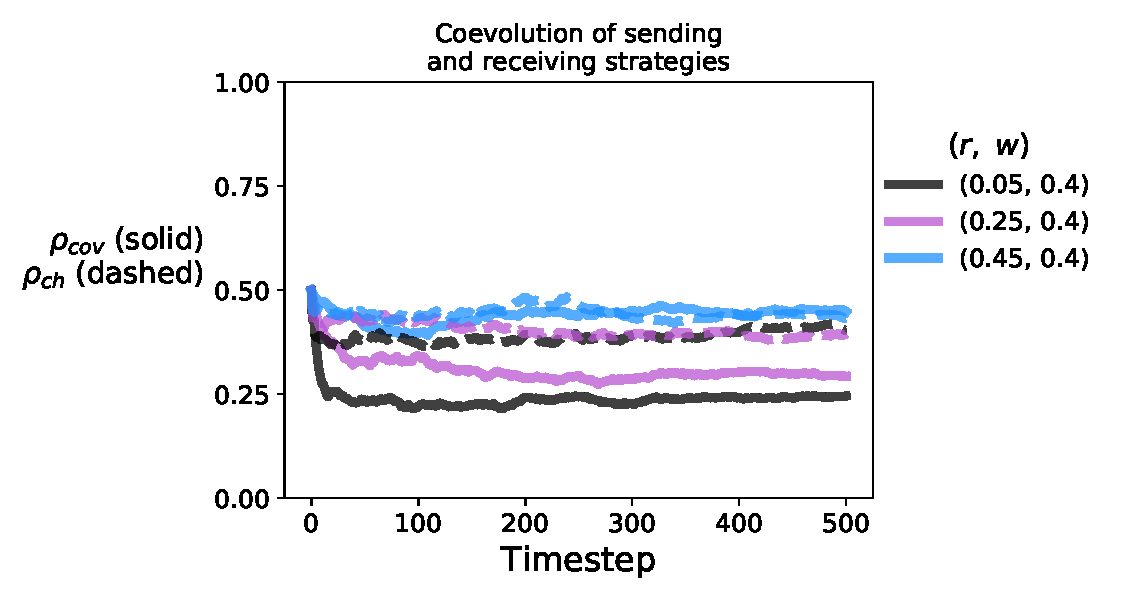
\includegraphics[width=\textwidth]{Figures/receptivity_evo_w=0p4.pdf}
  \caption{}
  \end{subfigure}
  \caption{Time series of communication strategy prevalences under different parameter settings
  for homophily, $w$, and covert signaling efficiency, $E_{cov}$.}
  \label{fig:}
\end{figure}

\subsubsection{Mean versus median outcomes}

Here I want to examine
\begin{enumerate}
  \item Histograms of the final distribution of prevalences for a number of
    parameter settings.
  \item Show time series of a selection (e.g. 10 or 20) of trials for a number
    of parameter settings to know that our averaged timeseries are showing
  typical behavior, not probabilities of an extreme outcome, i.e. $\rho_s=0,1$.

\end{enumerate}

\subsection{$d \neq \delta$}

Vary $\delta$ from 0 to $2d$.



\subsection{Invasion of other strategies}

In the main text we examined what conditions led to successful invasion of
the covert signaling strategy. Here in the supplement we analyze what
allows the other three strategies to invade: overt signaling, and churlish
and generous receiving.

\begin{figure}[H]
  \centering
  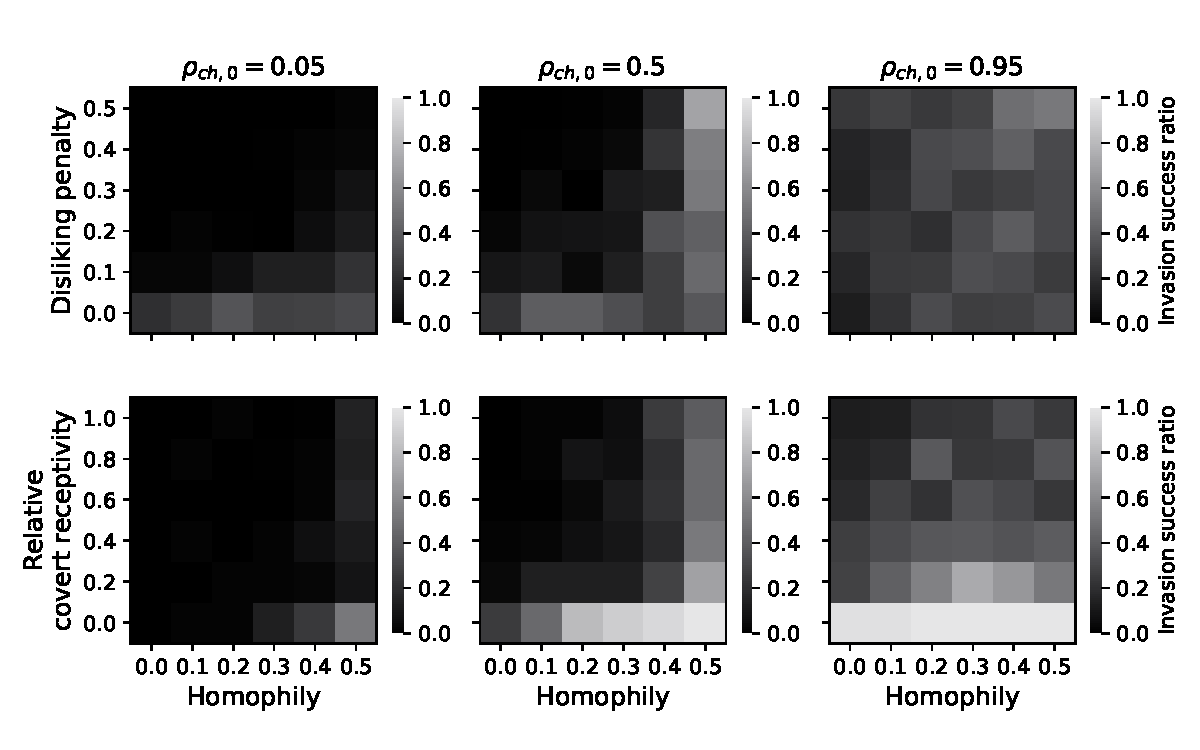
\includegraphics[width=\textwidth]{Figures/overt_invades.pdf}
  \caption{Overt invades, $\rho_{cov,0}=0.95$}
  \label{fig:ov-invades}
\end{figure}

\begin{figure}[H]
  \centering
    \begin{subfigure}{\textwidth}
      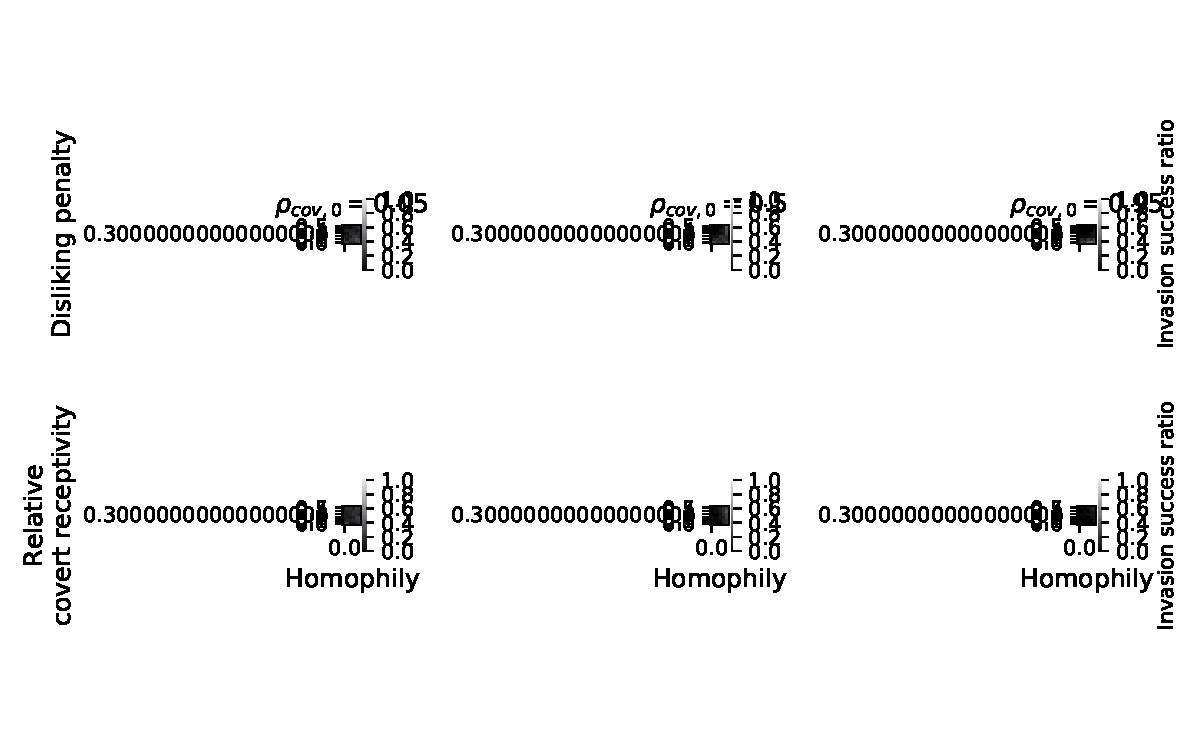
\includegraphics[width=\textwidth]{Figures/churlish_invades.pdf}
      \caption{Churlish invades, $\rho_{ch,0}=0.05$}
    \end{subfigure} \\
    \begin{subfigure}{\textwidth}
      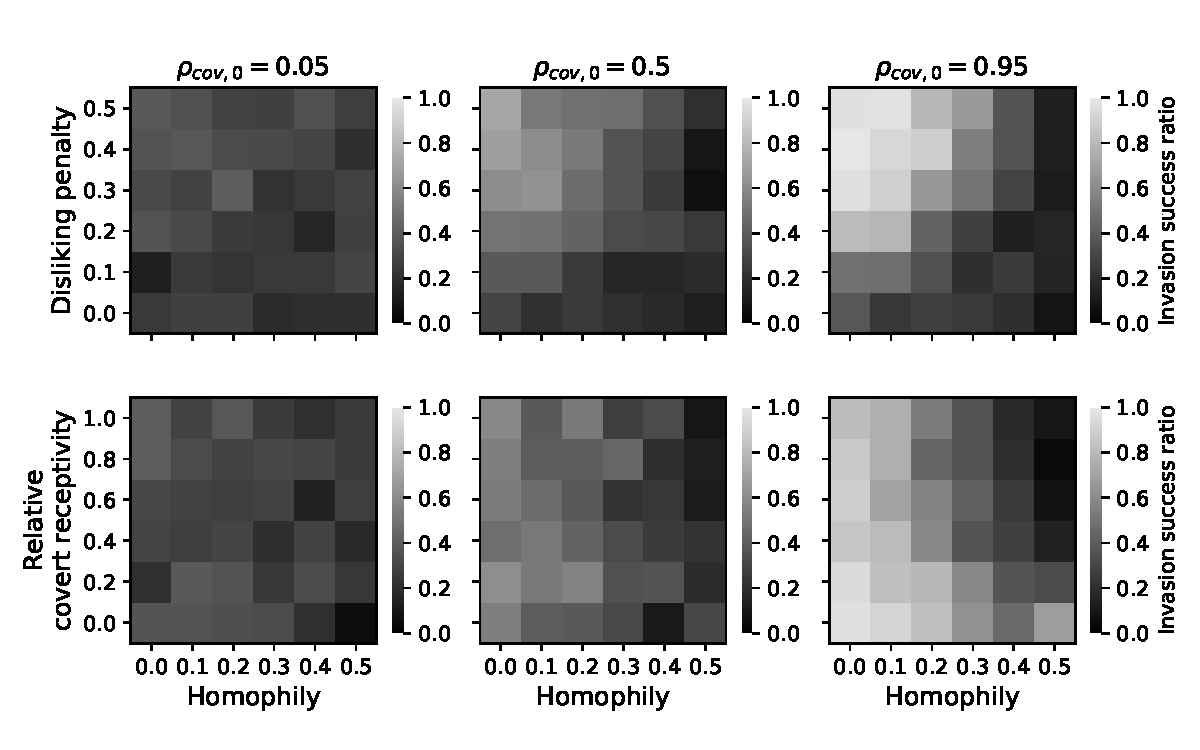
\includegraphics[width=\textwidth]{Figures/generous_invades.pdf}
      \caption{Generous invades, $\rho_{ch,0}=0.95$}
    \end{subfigure}
  \caption{Churlish and generous receiving strategy invasion success rates.
    For low to moderate rates of initial covert signaling there is not much
    of a pattern to invasion success. High values of homophily do seem to lead
    to more successful churlish invasion for moderate values of initial
    covert signalers. For large initial proportions of covert
    signalers, lower homophily favors generous invasion, which is more pronounced
    for larger disliking penalties.
  }
  \label{fig:ch-gen-invades}
\end{figure}

\subsection{Different learning parameters}

In the main text we have set the learning parameters to be $\alpha=1.25$ and
$\beta=12.0$. Setting $\alpha=1.25$ means that for there to be a 50\% chance
of the learner to match its strategy with its teachers, the teacher's 
accumulated payoff for that round must be 1.25 that of the learner's. This
seems somewhat severe, and we imagine that a different adoption threshold values
$\alpha$ could lead to different patterns in the spread of the covert signaling
strategy. In this section we test $\alpha=1.0$ (TO BEGIN WITH THEN WE WILL TEST
OTHER VALUES IF IT SEEMS VALUABLE TO DO SO).


\subsection{Different number of interaction rounds per model iteration}

One model iteration consists of a signalling round followed by $N_I$ interaction
rounds in which agents are matched randomly into dyads then collaborate 
with probability proportional to the attitudes each agent in the dyad has towards
the other (Equation~\ref{eq:homophily}). In the main text, $N_I = 10$ for
all experiments that generated the results we presented. 

\section{Model implementation}

In order to aid evaluation of our model code, we provide notes below on 
our model implementation. The code is freely available on GitHub at
\url{https://github.com/mt-digital/identity-signaling}.

\end{document}
